\documentclass{article}
% \usepackage{geometry}
% \geometry{left=3cm,right=3cm,top=2cm,bottom=2cm}
% \usepackage{neurips_2019}
\usepackage[utf8]{inputenc}
\usepackage[T1]{fontenc}
\usepackage{amsfonts}
\usepackage{nicefrac}
\usepackage{microtype}
\usepackage{float, array}
\usepackage{amssymb, amsmath, bm, amsthm}
\usepackage[caption=false,font=scriptsize]{subfig}
\usepackage[ruled,vlined]{algorithm2e}
\usepackage{enumerate}
\usepackage{graphicx}
\usepackage{color, colortbl}
\usepackage{epstopdf}
\usepackage{booktabs, multirow}
\definecolor{darkgreen}{rgb}{0, 0.5, 0}
\definecolor{red}{rgb}{1, 0, 0}
\usepackage{chngpage}

\usepackage{mfirstuc}
\usepackage{mathtools}
\usepackage{lettrine}
\usepackage{pxfonts}
\usepackage{epstopdf}
\usepackage{url}
\def\UrlBreaks{\do\/\do-}

\DeclareMathOperator*{\minimize}{minimize}
\DeclareMathOperator*{\maximize}{maximize}
\DeclareMathOperator*{\argmin}{argmin}
\DeclareMathOperator*{\argmax}{argmax}

\newcommand\etal{\textit{et al.}}
\newcommand\ie{\textit{i.e.}}
\newcommand\eg{\textit{e.g.}}
\newcommand\st{\textit{s.t.}}
\newcommand\wrt{\textit{w.r.t.}}
\newcommand\etc{\textit{etc.}}
\newcommand\doubleE{\mathbb{E}}
\newcommand\doubleP{\mathbb{P}}
\newcommand\doubleR{\mathbb{R}}
\newcommand\scriptS{\mathcal{S}}
\newcommand\scriptO{\mathcal{O}}
\newcommand\scriptA{\mathcal{A}}

\newtheorem{theorem}{Theorem}[section]
\newtheorem{fact}{Fact}[section]
\newtheorem{definition}{Definition}[section]
\newtheorem{proposition}{Proposition}[section]
\newtheorem{corollary}{Corollary}[section]
\newtheorem{lemma}{Lemma}[section]
\newtheorem{proofidea}{Proof Idea}[section]
\begin{document}
\title{Faster and More Accurate Learning with \\ Meta Trace Adaptation}
\author{
\begin{tabular}[t]{cc}
Mingde Zhao & Ian Porada
\end{tabular}
}
\date{ }
\maketitle
\begin{abstract}
Learning speed and accuracy are of universal interest for reinforcement learning problems. In this paper, we investigate meta-learning approaches for adaptation of the trace decay parameter $\lambda$ used in TD($\lambda$), from the perspective of optimizing a bias-variance tradeoff. We propose an off-policy applicable method of meta-learning the $\lambda$ parameters via optimizing a meta-objective with efficient incremental updates. The proposed trust-region style algorithm, under proper assumptions, is shown to be equivalent to optimizing the bias-variance tradeoff for the overall target for all states. In experiments, we validate the effectiveness of the proposed method MTA showing its significantly faster and more accurate learning patterns compared to the compared methods and baselines.
\end{abstract}

\section{Introduction}\label{sec:introduction}
Assembling the compound targets is an open problem for achieving good learning performance in Reinforcement Learning (RL). TD($\lambda$), which uses a single parameter controlled geometric sequence as the weights of the $n$-step returns, stands out from the sea of compound update methods for its efficient incremental updates and its interesting mathematical properties.
\par
Empirical studies show that different $\lambda$'s yield different performance. Furthermore, it is expected that adapting $\lambda$ appropriately during the learning boosts performance in terms of convergence speed and accuracy.
\par
The goal of this paper is to find a method that optimizes the overall target error for all the states. We first derive a new state meta-objective for optimizing the bias-variance tradeoff and show that the meta-objective proposed in an existing work \cite{white2016greedy} is actually a special case of the newly proposed objective. Then, we propose a trust-region style method to tackle the difficulties of optimizing the meta-objective and prove its equivalence to optimizing the overall target error, given appropriate assumptions. In experiments, we observe that the proposed method MTA has generally significantly improved empirical performance over the existing method and baselines.

\section{Preliminaries}\label{sec:preliminaries}
TD($\lambda$) \cite{Singh1996} is a TD learning variant which uses a weighted combination of the multi-step targets as the update target, which is called the $\lambda$-return. The weights constitute a geometric sequence controlled by the hyperparameter $\lambda \in [0, 1]$ and are applied from the $1$-step return to the $\infty$-step return (MC return). TD($\lambda$) became popular for its so-called ``backward view'', which means that the updates towards the $\lambda$-return can be approximated in a fully incremental manner with space and time complexity $\scriptO(n)$\footnote{$n \equiv |S|$, the number of states in the state space $|\scriptS|$.} using buffer vectors called the ``eligibility traces''. Eligibility traces are not only attractive for its computational efficiency and ease of implementation, but also for their interesting mathematical properties.
\par
Despite great success, this family of TD($\lambda$) has been haunted by the fact that the incremental updates can only \textit{approximate} the true $\lambda$-return. Only recently, researchers have present a ``truely online'' approach, which shows that it is possible to use auxiliary vectors to make the updates exactly equivalent to update towards a true $\lambda$-return. The true online algorithms also bring the possibility of \textit{fully} controlling the bias-variance tradeoff during the learning process by adapting $\lambda$.

\subsection{The Trace Adaptation Problem}
% We consider the typical RL setting in which the environment is defined by a markov decision process (MDP) with state space $\scriptS$, action space $\scriptA$, reward function $r: \scriptS \times \scriptA \times \scriptS \to \doubleR$, and state-based discount factor $\gamma : \scriptS \to [0, 1]$\footnote{This is a generalized setting compared to fixing the discount factor $\gamma$ for all states.}. We are then concerned with policy evaluation, which amounts to finding the true value function $j: \scriptS \to \doubleR$ that is defined to be the expectation of the discounted return starting at state $s \in \scriptS$ and following policy $\pi: \scriptS \times \scriptA \to [0, 1]$.
% \par
When the environment MDP is not known and we are using some form of the TD($\lambda$) algorithm for policy evaluation (for a fixed policy), we can adjust the hyperparameter $\lambda$ according to the experiencing state, \st{} the learning speed is accelerated and the final error of the value function (in terms of $L_2$-distance) is minimized. The problem we address is how exactly to adjust $\lambda$ to achieve such a goal.
\par
Research into $\lambda$ adaptation is really research into the ways of making use of the information available to adapt $\lambda$. A promising direction is to derive state based $\lambda$'s as time-dependent adaptions are considered as not equipped with a well-defined fixed point \cite{white2016greedy}. Thus, in this paper, we seek only to find a congenial (\ie{} incremental and online), state-dependent adaptation for $\lambda$.
\par
$\lambda$ is a hyper-parameter, so we will require a meta-adaptation mechanism to change it. An adaptive hyper-parameter method differs from traditional hyper-parameter tuning in that the selection of the hyper-parameter is an active part of the training process. Thus adaptive lambda can potentially outperform any static lambda method while also not requiring the additional sample complexity necessary for hyper-parameter tuning.
\par
Much research has gone into meta-learning the learning rate hyper-parameter in temporal difference algorithms \cite{dabney2012adaptive}, while investigations into meta-learning the trace parameter are fairly limited. The majority of existing methods for $\lambda$ adaptation do not work in the incremental backwards view due to their design or computational complexity \cite{kearns2000bias, schapire1996worst, singh1997analytical, konidaris2011td_gamma}. More recently, there has been success in adaptively selecting a state-based lambda using inaccurate estimates of Monte Carlo return's expectation and variance \cite{white2016greedy}. This technique serves as the basis of our contribution, and we use this method as a baseline in our analyses.
\input{tab_notations.txt}
\subsection{Background Knowledge}
Here we provide some background knowledge for understanding the contexts of this paper. Before that, we present all the notations in Table \ref{tab:notations}.

% \begin{definition}[Return]
% The \textbf{generalized discounted return} (\textbf{return}) is the discounted sum of future rewards
% \begin{equation}
% G_t \equiv R_{t+1} + \gamma_{t+1} R_{t+2} + \gamma_{t+1}\gamma_{t+2} R_{t+3} + \cdots = R_{t+1} + \gamma_{t+1}G_{t+1}
% \end{equation}
% \end{definition}
% The discount function $\gamma: \mathcal{S} \to [0, 1]$, with $\gamma_t \equiv \gamma(S_t)$, provides a variable level of discounting depending on the state \cite{sutton2011horde}.
% \par
% \subsubsection{Temporal-difference Learning}
% Temporal-Difference (TD) learning is the most fundamental idea of incremental RL. Its intuition can be described as ``learning a guess from a guess'': each update combines the truth observed from the environment and the current estimates.
% \begin{fact}[$1$-step TD Convergence]
% The $1$-step TD update rule $J(S_t) \leftarrow R_{t+1} + \gamma_{t+1} J(S_{t+1})$ achieves asymptotic convergence to the true value $j(S_t)$ with enumerating state representations, where $J(S_t)$ is the estimated value function and $j(S_t)$ is the true value function.
% \end{fact}
% The reason why TD methods can achieve convergence in the tabular case is that, if we consider this as an operator, we can prove its contraction property and can find that the guaranteed fixed-point is the true value function.
% \par
% The Bellman operator \cite{DBLP:books/lib/SuttonB98} serves as a contraction on our estimate of the return to some fixed point.
% \begin{definition}[Bellman Operator]
% $B_\pi : \mathbb{R}^{|\mathcal{S}|} \to \mathbb{R}^{|\mathcal{S}|}$
% \begin{equation}
% \begin{aligned}
%     (B_\pi j)(S_t) = \sum_{A_{t}} \pi(A_t | S_t) \sum_{S_{t+1}, R_{t+1}} p(S_{t+1}, R_{t+1} | S_t, A_t) [R_{t+1} + \gamma(S_{t+1}) j(S_{t+1})]
% \end{aligned}
% \end{equation}
% \end{definition}


% \begin{theorem}[Banach's Fixed Point]\label{thm:fixed_point}
% % \textcolor{red}{Fixed-point existence, convergence, contraction}
% For a contraction mapping $T: X \to X$ there exists a unique fixed point $x \in X$ \st{} $T(x) = x$.
% \end{theorem}

% The Bellman operator for the estimation of values is a contraction and that is how we get the guarantees that the TD algorithms will work (in cases with well defined fixed point, \eg{} tabular). The theorem also indicates that, if a Bellman operator of some any statistic is a contraction and the fixed point exists, we are guaranteed to successfully estimate such statistics using the respective Bellman operator.

Asymptotic convergence in the tabular case is not always useful in practice: we can never afford infinite number of episodes nor can we apply this onto environments with the numbers of states too large to be enumerated, \eg{} continuous state spaces. However, with limited number of episodes or function approximations, we lose most of the convergence guarantees. Thus in the cases with no theoretical analyses, we have to know how to evaluate the quality of a given estimate for the value function.

\begin{definition}[Mean Squared Error for Value Function]
Given the true value function $\bm{j}$ and its estimate $\bm{J}$ of target policy $\pi$, the \textbf{mean squared error} for $\bm{J}$ or \textbf{value error}is defined as:
$$MSE(\bm{J}) = {\| D \cdot (\bm{J} - \bm{j}) \|}_2^2$$
where $D \equiv diag(d_\pi(s_1), d_\pi(s_2), \cdots, d_\pi(s_{|S|}))$ and $d_\pi(s_i)$.
\end{definition}
\par
The Mean Squared Error (MSE) for value function is a weighted $L_2$-distance between the true value $\bm{j}$ and its estimate $\bm{J}$. The weights favor the states that the agent will meet with higher frequency under the policy.
\par
\begin{definition}[Mean Squared Error for Target]
Given the true value function $\bm{j}$ and the update target $\bm{G}$, the \textbf{mean squared error} for $\bm{G}$ for estimate $J$ or \textbf{target error} is defined as:
$$MSE(\bm{G}) = {\| D \cdot (\doubleE[\bm{G}] - \bm{j}) \|}_2^2$$
\end{definition}
\par
The MSE for target measures the distance between the update target of the value estimates and the true value function. The closer they are, the better target the value estimate is updated towards.

\subsubsection{Multi- and Compound-TD \& TD($\Lambda$)}
\begin{definition}[$n$-step Return]
For trajectory $\tau: S_t \to \cdots \to S_T$, the \textbf{$n$-step return} is defined as:
$$G_t^{(n)} \equiv R_{t+1} + \gamma_{t+1}R_{t+2} + \cdots + \prod_{i=t+1}^{n-1}{\gamma_{i}}R_{t+n} + \prod_{i=t+1}^{n}{\gamma_{i}}J_{t+n-1}(S_{t+n})$$
\end{definition}
% $n$-step returns become the one step TD return when we set $n = 1$ and the MC return for $n = \infty$. $1$-step TD and MC can be seen as the two extreme cases for multi-step TD learning.
\begin{fact}[Compound Update]
Any TD updates using a convex combination of the $n$-step returns as the target is called a \textbf{compound update}. In tabular cases, compound updates have guarantee of convergence to the correct value estimates under appropriate conditions. With certain function approximators, certain type of compound updates also have convergence guarantees.
\end{fact}

TD($\Lambda$) can be viewed as a variant of the multi-step TD algorithm. For the update of each state, TD($\Lambda$) uses a particular $\lambda$ to create a geometric sequence of weighting for the $n$-step returns. It interpolates between TD($0$) and Monte-Carlo, achieving generally better learning speed and accuracy than the individual multi-step methods. To have convergence guarantees with linear function approximators\footnote{GTD methods is for linear approximators only. For more complicated function approximators, we do not have well-defined fixed points for the Bellman operators and thus cannot have the guarantees.}, we use the TD($\Lambda$) variant Gradient TD($\Lambda$) (GTD($\Lambda$)) \cite{sutton2009convergent, sutton2009fast}.
\begin{definition}[$\Lambda$-return]
The generalized $\Lambda$-return $G_t^\Lambda$, where $\Lambda \equiv \{\lambda_1 \equiv \lambda(S_1), \lambda_2 \equiv \lambda(S_2), \dots, \lambda_t \equiv \lambda(S_t), \dots\}$, from one state $S_t$ in a trajectory $\tau$ is defined as
\begin{equation}
G_t^\Lambda \equiv G^\Lambda(s_t) = R_{t+1} + \gamma_{t+1} [(1 - \lambda^{(t+1)})J(s_{t+1}) + \lambda^{(t+1)}G_{t+1}^\Lambda]
\end{equation}
where $G_t^\Lambda = 0$ for $t > |\tau|$.
\end{definition}
This is a generalized definition for state dependent $\lambda$'s. When $\lambda$ is the same across the time-steps for all states, this becomes the classic $\lambda$-return. The $\Lambda$-return is a specific type of compound return, which is used in (generalized) TD($\Lambda$).
\par
% TD($\Lambda$) defines the $\Lambda$-return for a state pretending to know all the future rewards, which means one probably has to wait until the end of the episode to calculate the $\Lambda$-return, \ie{} it seems to have to be calculated offline. However, that is not the case: TD($\Lambda$) can be approximated by computationally congenial\footnote{Meaning that for each step the agent takes online in the environment, it consumes approximately equal computational power \cite{DBLP:books/lib/SuttonB98}} incremental updates online! To show such possibility, we start from the classical TD($\lambda$) with fixed $\lambda$.
% \begin{proposition}[classical Trace Approximation]
% When the trajectory is infinitely long, the updates using (classic) $\lambda$-return as targets can be approximated using eligibility traces incrementally.
% \end{proposition}
% \begin{proof}
% \begin{equation}
% \begin{aligned}
% & G_t^\lambda - J(S_t)\\
% & = -J(S_t) + (1 - \lambda) \lambda^0 (R_{t+1} + \gamma^1 J(S_{t+1})) + (1 - \lambda) \lambda^1 (R_{t+1} + \gamma^1 R_{t+2} + \gamma^2 J(S_{t+2})) + \cdots\\
% & = -J(S_t) + (1 - \lambda)[\lambda^0\gamma^0(\lambda^0 + \lambda^1 + \cdots)R_{t+1} + \lambda^1\gamma^1(\lambda^0 + \lambda^1 + \cdots)R_{t+2} + \cdots + \gamma^1\lambda^0 J(S_{t+1}) + \gamma^2\lambda^1 J(S_{t+2}) + \cdots]\\
% & = -J(S_t) + (1 - \lambda)[\frac{\lambda^0\gamma^0}{1-\lambda}R_{t+1} + \frac{\lambda^1\gamma^1}{1-\lambda}R_{t+2} + \cdots + \gamma^1\lambda^0 J(S_{t+1}) + \gamma^2\lambda^1 J(S_{t+2}) + \cdots]\\
% & = (\gamma \lambda)^0(R_{t+1} + \gamma J(S_{t+1}) - \gamma \lambda J(S_{t+1})) + (\gamma \lambda)^1(R_{t+2} + \gamma J(S_{t+2}) - \gamma \lambda J(S_{t+2})) + \cdots\\
% & = \sum_{k=t}^{\infty}{(\gamma \lambda)^{k-t}(R_{k+1} + \gamma J(S_{k+1}) - J(S_k))}
% \end{aligned}
% \nonumber
% \end{equation}
% This is exactly the form of accumulating trace\footnote{People refer to ``eligibility'' trace as the family of the algorithms that employ trace vectors to incrementally approximate something that cannot be calculated directly. There are several variants of the eligibility traces. The accumulating traces are the original and the most classical one.}:
% $$\bm{z}^{(t)} = \gamma \lambda \bm{z}^{(t-1)} + \bm{\nabla} J(\bm{x}_{t}, \bm{w}^{(t)})$$
% $$\bm{w}^{(t+1)} = \bm{w}^{(t)} + \alpha [R_{t+1} + \gamma J(\bm{x}_{t+1}, \bm{w}^{(t)}) -J(\bm{x}_{t}, \bm{w}^{(t)})] \bm{z}^{(t)}$$
% \end{proof}

\begin{fact}[$\Lambda$ Trace Approximation]
With an infinitely long trajectory, the updates using the $\Lambda$-return as targets can be approximated using eligibility traces incrementally with the update rules:
$$\bm{z}^{(t)} = \gamma_t \lambda^{(t)} \bm{z}^{(t-1)} + \bm{\nabla} J(\bm{x}_{t}, \bm{w}^{(t)})$$
$$\bm{w}^{(t+1)} = \bm{w}^{(t)} + \alpha [R_{t+1} + \gamma_t J(\bm{x}_{t+1}, \bm{w}^{(t)}) - J(\bm{x}^{t}, \bm{w}^{(t)})] \bm{z}^{(t)}$$
\end{fact}

% \begin{proof}
% \begin{equation}
% \begin{aligned}
% & G_t^\Lambda - J(S_t)\\
% & = -J(S_t) + R_{t+1} + \gamma_{t+1}(1 - \lambda^{(t+1)})J(s_{t+1}) + \gamma_{t+1}\lambda^{(t+1)}G_{t+1}^\Lambda\\
% & = -J(S_t) + R_{t+1} + \gamma_{t+1}(1 - \lambda^{(t+1)})J(s_{t+1}) + \gamma_{t+1}\lambda^{(t+1)}(R_{t+2} + \gamma_{t+2}(1 - \lambda^{(t+2)})J(s_{t+2}) + \gamma_{t+2}\lambda^{(t+2)}G_{t+2}^\Lambda)\\ & = -J(S_t) + R_{t+1} + \gamma_{t+1}(1 - \lambda^{(t+1)})J(s_{t+1}) + \gamma_{t+1}\lambda^{(t+1)}R_{t+2} + \gamma_{t+1}\lambda^{(t+1)}\gamma_{t+2}(1 - \lambda^{(t+2)})J(s_{t+2}) + \gamma_{t+1}\lambda^{(t+1)}\gamma_{t+2}\lambda^{(t+2)}G_{t+2}^\Lambda\\
% & = \cdots\\
% & = \sum_{k=t}^{\infty}{(\gamma_k \lambda^{(k)})^{k-t}(R_{k+1} + \gamma_k J(S_{k+1}) - J(S_k))}
% \end{aligned}
% \nonumber
% \end{equation}
% \end{proof}
% This leads to the backward approximation rule of generalized TD($\Lambda$):
\par
The possibility for accumulating generalized traces ensures the viability of state based $\lambda$. We call this operation ``meta trace adaptation'' if we use meta approaches to learn to adapt the traces used in the incremental updates in TD($\Lambda$).
\par
The incremental approximation of updates using $\Lambda$-returns as targets is often recognized as the ``backward view'', while the updates based on $\Lambda$-return is often recognized as the ``forward view''. Though it is called the backward view, it is actually done in the same direction as time without having to look back in time.
\par
Nevertheless, it should also be noticed that the proposition is proved based on the assumption that the trajectory is infinitely long. For the finite length trajectory, this is only roughly equivalent. We should realize that the return or $\Lambda$-return for an infinitely long trajectory is confusing: the infinite length trajectories are infeasible for many cases. So we have to find an exact incremental equivalence to the updates using $\Lambda$-returns as targets. This has been an open-problem until the emergence of the so-called ``true online'' algorithms \cite{seijen2015true}, which use slightly more complicated incremental updates to achieve true equivalence to the $\Lambda$-return with linear function approximators. The true equivalence gives us the full control of the $\Lambda$-return.
% \begin{fact}[True Online Equivalence]
% The following incremental update rules achieve exact equivalence to updates using $\Lambda$-return targets using linear function approximations:
% $$\delta_t = R_{t+1} + \gamma_{t+1} \bm{x}_{t+1}^T w_{(t)} - \bm{x}_{t}^T w_{(t)} $$
% $$\bm{z}_{(t)} = \gamma_{t}\lambda_{(t)}\bm{z}_{(t-1)} + \bm{x}_{t} - \alpha\gamma_{t+1}\lambda_{(t+1)}(\bm{z}_{(t)}^T\bm{x}_{t})\bm{x}_{t}$$
% $$\bm{w}_{(t+1)} = \bm{w}_{(t)} + \alpha \delta_t \bm{z}_{(t)} + \alpha (\bm{w}_{(t)}^T \bm{x}_t - \bm{w}_{(t-1)}^T \bm{x}_t)(\bm{z}_{(t)} - \bm{x}_t)$$
% where $\alpha$ is the step-size hyperparameter that is consistent from both the forward view and the backward view.
% \end{fact}
\par
\begin{fact}[Fixed-point for Offline GTD($\Lambda$)]
Offline GTD($\Lambda$) with linear function approximation converges to fixed-points defined with $\Lambda$.
\end{fact}
The exact equivalence gives us the possibility of provably achieving a fixed point and adjusting the fixed point towards better performance. In this paper, we develop our ideas upon the true online GTD method, which combines the merits of being truely online and gradient based \cite{hasselt2014true}, to achieve survival of the deadly triad and the full control of the bias-variance tradeoff, \st{} with guarantees we can focus on the meta trace adaptation. The pseudocode of true online GTD($\Lambda$) is provided and presented in the appendices.

% However, this is not enough, since we would want an algorithm that works also on the off-policy case, in which the target policy to be evaluated is different from the behavior policy that controls the actions of the agent. This leads us to the famous problem of the deadly triad.
% \subsubsection{Deadly Triad}
% The danger of instability and divergence arises whenever we combine all of the following three elements, making up what we call the ``deadly triad'':
% \begin{enumerate}
% \item Function approximation: A powerful, scalable way of generalizing from a state space much larger than the memory and computational resources (\eg{} linear function approximation or NNs);
% \item Bootstrapping: Update targets that include existing estimates (as in dynamic programming or TD methods) rather than relying exclusively on actual rewards and complete returns (as in MC methods);
% \item Off-policy training: Training on a distribution of transitions other than that produced by the target policy. Sweeping through the state space and updating all states uniformly, as in dynamic programming, does not respect the target policy and is an example of off-policy training.
% \end{enumerate}
% \par
% Note that the danger is not due to control or to generalized policy iteration. Those cases are more complex to analyze, but the instability arises in the simpler prediction case whenever it includes all three elements of the deadly triad. The danger is also not due to learning or to uncertainties about the environment, because it occurs just as strongly in planning methods, such as dynamic programming, in which the environment is completely known.
% \par
% If any two elements of the deadly triad are present, but not all three, then instability can be avoided.
% \par
% The problem of the deadly triad has haunted the RL field for years until recently, there emerged a family of gradient based methods based on linear function approximation that provably survive the deadly triad, known as the GTD methods.
% \par
% GTD has good theoretical properties, but has lower convergence speed than the ordinary TD method.
\par
How are we going to learn faster and achieve better accuracy by changing $\Lambda$? We shall first review a principled approach with good empirical performance, which is proposed in \cite{white2016greedy}.

\subsection{$\lambda$-Greedy}\label{sec:whites}
Before the $\lambda$-greedy method, there were no meta-learning methods for $\lambda$ that could achieve incremental updating, compatibility with function approximation and stability during both on- and off-policy learning. White and White \cite{white2016greedy} proposed a novel objective function, which we will refer to as the ``greedy state meta-objective'' or ``greedy objective'' for optimizing $\lambda$ as a function of states and proposed several necessary components for the meta-optimization.

\subsubsection{The Greedy State Meta-objective}
For the optimization of the MSE of the target policy, they claimed that jointly optimizing the overall MSE for all states is not feasible, and thus took a greedy approach: for each time step, select $\lambda^{(t+1)} \equiv \lambda(s_{t+1})$ to optimize the bias-variance tradeoff for only the state that the agent is going to experience at the next step, \ie{} $S_t$. This greedy objective corresponds to minimizing the MSE between the unbiased $\lambda = 1$ return $G_t$ and the estimate $\hat{G}_t$ with $\lambda^{(t+1)} \in [0, 1]$ and $\lambda_{(k)} = 1, \forall k \geq t + 2$ into the future.
$$\hat{G}_t \equiv \rho_t(R_{t+1} + \gamma_{t+1} [(1 - \lambda^{(t+1)})J(\bm{x}_{t+1}, w_v^{(t+1)}) + \lambda^{(t+1)} G_{t+1}])$$
\par
We will provide an interpretation of such formulation later. $\hat{G}_t$ interpolates between the current value estimate $J(\bm{x}_{t+1}, \bm{w}^{(t+1)})$ and the unbiased MC return. The approach is to greedily decide how $\lambda^{(t+1)}$ should be set on this step to locally optimize the MSE, \ie{} bias and variance. This greedy decision is made given both $\bm{x}_t$ and $\bm{x}_{t+1}$, which are both available.
\begin{proposition}[Minimizer of Greedy Objective]\label{prop:greedy_minimizer}
Given the update target $\hat{G}_t$ of state $s$, the minimizer $\lambda_{(t+1)}^*$ of the mean squared target error of the state
$MSE \equiv \doubleE[{(\hat{G}_t - \doubleE[G_t])}^2]$ is:
\begin{equation}\label{eq:white_argmin}
\lambda_{(t+1)}^* = \frac{{err}^2(\bm{w}^{(t)}, \bm{x}_{t+1})}{Var[G_{t+1}] + {err}^2(\bm{w}^{(t)}, \bm{x}_{t+1})}
\end{equation}
where $err(\bm{w}, \bm{x}_{t+1}) \equiv \doubleE[G_{t+1}] - J(\bm{x}_{t+1}, \bm{w}^{(t)})$.
\end{proposition}
The proof is in the appendices. This is elegant and always feasible unless both variance and error are $0$, in which case any choice of $\lambda$ is the same. To get the approximate solution of the optimization problem, we must estimate $Var[G_{t+1}]$ effectively.

\subsubsection{VTD \& DVTD}
In \cite{white2016greedy}, VTD is proposed as a method of estimating the variance of the MC return alongside the TD updates by further decomposing $Var[G_{t+1}] = \doubleE[G_{t+1}^2] - \doubleE^2[G_{t+1}]$ and estimating the second and the first moments separately.
\par
% \par
% Though the algorithm only needs the estimation of the MC return, which is the $\Lambda$-return with $\Lambda = 1$, the authors provided a general model-free estimation approach of the second moment of the $\Lambda$-return.
% \par
% The recursive form for the squared $\Lambda$-return is
% \begin{equation}
% \begin{aligned}
% (G_t^\Lambda)^2 & = \rho_t^2 (R_{t+1} + \gamma_{t+1} [(1 - \lambda^{(t+1)})J(s_{t+1}) + \lambda^{(t+1)}G_{t+1}^\Lambda])^2\\
% & = \rho_t^2 \left( (R_{t+1} + \gamma_{t+1}(1 - \lambda^{(t+1)})J(s_{t+1})) + \gamma_{t+1}\lambda^{(t+1)}G_{t+1}^\Lambda \right)^2 \equiv \overline{r}_{t+1} + \overline{\gamma}_{t+1}(G^{\Lambda}_{t+1})^2
% \end{aligned}
% \end{equation}
% where $\overline{\gamma}_{t+1} \equiv \rho_t^2 \gamma_{t+1}^2 \lambda_{(t+1)}^2$, $\overline{r}_{t+1} \equiv \rho_t^2 \overline{G}_t^2 + 2\rho_t^2 \gamma_{t+1}\lambda^{(t+1)} \overline{G}_t G_{t+1}^\Lambda$ and
% $\overline{G}_t \equiv R_{t+1} + \gamma_{t+1}(1 - \lambda^{(t+1)})J(s_{t+1})$.
% \par
% The recursive form of $(G_t^\Lambda)^2$ is similar to that of the $\Lambda$-return. If we write it in exactly that form, we can have the possibility of estimating the second moment alongside the first moment:
% $$\overline{J}_t^{\overline{\Lambda}} \equiv \overline{r}_{t+1} + \overline{\gamma}_{t+1}\left((1-\overline{\lambda}^{(t+1)})J(\bm{x}_{t+1}, \bm{w}_{SQ}^{(t)}) + \overline{\lambda}^{(t+1)} \overline{J}_{t+1}^{\overline{\Lambda}} \right)$$
% This introduces a meta-parameter $\overline{\lambda}^{(t+1)}$. $(G_t^\Lambda)^2$ can be estimated by setting $\overline{\lambda}^{(t+1)} = 1$.
This is great since the variance of $\Lambda$-return can be estimated alongside the first moment. But only showing this is not enough for convergence guarantees, which will require showing the corresponding Bellman operator to be a contraction. By restricting to the linear case in GTD, the contraction of such Bellman operator is proved and the update rule for using GTD is derived\footnote{Details to be found in \cite{white2016greedy}.}.

% \begin{figure}
% \centering
% \includegraphics[width = 0.65\textwidth]{}\\
% \caption{Reproduction of the Whites' experiment for $11$ state ring world ($\gamma = 0.95$). The target policy takes action left with probability $0.05$ while the behavior policy takes action left with probability $0.15$. The experiments are run $40$ times independently with each $1000$ episodes. It can be seen that the greedy method has similar performance to MC, which shows its effectiveness in such test case.}
% \label{fig:greedy_off}
% \end{figure}

% Why we have to be skeptical? The sample efficiency will always be an issue!

% Why does the Whites \cite{white2016greedy} use GTD \cite{sutton2009convergent}? GTD survives the deadly triad! Actually there is a family of GTD algorithms, check GTD, GTD2 \cite{sutton2009fast} and TDC \cite{sutton2009fast}.

% Why don't they use true online TD \cite{seijen2015true}?

% Can Whites' method be extended to any kind of function approximation methods? No provable convergence for more complicated type of function approximators.
\par
Sherstan \etal{} recently contributed a Bellman operator for directly estimating the variance of the $\Lambda$-return, named the DVTD, together with the guarantees \cite{sherstan2018directly}. Empirically, DVTD shows more robust performance than the VTD method that decomposes the variance into the difference between the second moment and the squared first moment, since the variance is only equivalent to the difference between the true second moment and the squared true first moment, not their estimates. We may achieve better performance on Whites' method by replacing VTD with the direct method. But, can we achieve more?

\section{MTA: Meta Trace Adaptation with True Objectives}\label{sec:MTA}
\par
In this section, we will derive the our novel meta-learning approach for trace adaptation. Different from the greedy objective, the meta-objective we offer aims at decreasing the overall MSE between the $\Lambda$-return target and the true value. We will first derive the ``true'' state meta-objective for each state.

\subsection{Meta-objective}
The greedy objective for each time-step tries to optimize the objective of a simplified $\Lambda$-return in which $\lambda^{(k)} = 0$ for $\forall k \geq t+2$. Though this objective shows very good empirical performance, it is far from the ``true'' objective that the learning algorithm wants to achieve. The true objective is to achieve lowest overall MSE \wrt{} the stationary distribution of the target policy.
\par
Such goal is considered to be generally infeasible. Here, we first derive the true state meta-objective\footnote{To be called the ``true objective'' for convenience.} for every state encountered in a trajectory, then we show the characteristics of the true objective and give our interpretation on the greedy objective. After that, we give our method of optimizing the true objective. And most excitedly, we will show that optimizing the true state objectives is equivalent to optimizing the overall target error.
\par
Now let us start with optimizing the target, \ie{} the $\Lambda$-return, for the current time step $t$ and the state $s_t$.
\begin{proposition}[Gradient of True Objective]\label{prop:objective}
Given the update target $G_t^\Lambda$ of state $s$, the gradient of the mean squared target error of the state $MSE \equiv \doubleE[(G_t^\Lambda - \doubleE[G_t])^2]$ is:
\begin{equation}
    \begin{aligned}
    & \nabla_{\lambda^{(t+1)}} \frac{1}{2} MSE(\lambda^{(t+1)}) = \\
    &\gamma_{t+1}^2 \left[\lambda^{(t+1)} \left[ (J(s_{t+1}) - \doubleE[G_{t+1}^\Lambda])^2 + Var[G_{t+1}^\Lambda] \right] + J(s_{t+1})(\doubleE[G_{t+1}^\Lambda] + \doubleE[G_{t+1}]) - J^2(s_{t+1}) - \doubleE[G_{t+1}^\Lambda]\doubleE[G_{t+1}]\right]
    \end{aligned}\nonumber
\end{equation}
And its minimizer is:
\begin{equation}
\begin{aligned}
& \argmin_{\lambda^{(t+1)}}{MSE(\lambda^{(t+1)})} = \frac{J^2(s_{t+1}) + \doubleE[G_{t+1}^\Lambda]\doubleE[G_{t+1}]-J(s_{t+1})(\doubleE[G_{t+1}^\Lambda] + \doubleE[G_{t+1}])}{(J(s_{t+1}) - \doubleE[G_{t+1}^\Lambda])^2 + Var[G_{t+1}^\Lambda]}
\end{aligned}\nonumber
\end{equation}
\end{proposition}
The proof is in the appendices. The solution of the true objective is a generalization of the greedy objective, since if we set $G_{t+1}^\Lambda = 0$, we get the closed-form solution of the greedy objective (\ref{eq:white_argmin}). However this is more complicated than the minimizer of the greedy objective: we need the estimate of $\doubleE[G_{t+1}]$, $\doubleE[G_{t+1}^\Lambda]$ and $Var[G_{t+1}^\Lambda]$, while for the simplified version we only need the estimation of $\doubleE[G_{t+1}]$ and $Var[G_{t+1}]$. Furthermore, if some $\lambda^{(t+1)}$ is changed, the estimates $\doubleE[G_{t+1}^\Lambda]$ and $Var[G_{t+1}^\Lambda]$ will be destroyed and will have to be re-estimated from scratch, since they depend on the whole $\Lambda$. While the estimate in for the greedy objective is invariant to the change of $\Lambda$. This is our interpretation for the reason why the greedy objective is crafted this way: though highly biased towards the MC return, it is with more stable estimates to calculate the optimal $\lambda$'s.
\par
% Though we have the Bellman operators to estimate these statistics, the true greedy objective can be very unstable if we greedily change any $\lambda^{(t+1)} \in \Lambda$, so what is the point of using this objective? It would be disaster if, the algorithm destroys all the estimates to change only one $\lambda^{(t+1)}$. So why not just use the simplified greedy objective instead anyway? We show that a different manner of adapting $\lambda$ results in something very interesting:
Though we have the means \cite{sherstan2018directly} to estimate these statistics, \ie{} $\doubleE[G_{t+1}]$, $\doubleE[G_{t+1}^\Lambda]$ and $Var[G_{t+1}^\Lambda]$, the true objective can be very unstable if we naively change any $\lambda^{(t+1)} \in \Lambda$: inappropriate change of $\lambda$ would potentially destroy all estimates. So why not just use the simplified greedy objective? Is there any benefit to use the true objective that seems infeasible to optimize? We show the following theorem:

\begin{theorem}[Achievement of Optimizing Overall Target Error]\label{thm:nongreedy}
Given an MDP, gradient descent on the true greedy objectives is equivalent to stochastic gradient descent on the overall target MSE for the expected $\Lambda$-return for policy $\pi$, with the assumption that the estimated statistics are accurate. More specifically:
$$\nabla_{\Lambda} \frac{1}{2} MSE(\Lambda) \approx \sum_{s \sim b}{\rho_{acc} \cdot \frac{1}{2} \nabla_{\lambda(s)} MSE(\lambda(s))}$$
where $s$ is the state that the agent is currently experiencing when rolling out behavior policy $b$, $\rho_{acc}$ is the product of all the importance sampling ratios from the beginning of the current episode until meeting state $s$.
\end{theorem}
The theorem shows that, combined with the importance sampling ratio, if we do gradient descent correctly on the true state meta-objectives, we will be actually optimizing on the true meta-objective. Correct gradient descent requires  a way to stabilize the estimates: if we have that, we are going to lead $\Lambda$ to a minimum of the bias-variance tradeoff of overall target error.
\par
But how? We use a trust region method: the true state meta-objective is continuous (constituted of squared bias and variance), a very small gradient descent step in $\lambda^{(t+1)}$ is only going to result a bounded shift of the estimates. This means that if we use a small enough step size of gradient descent to change $\lambda$, we can actually stabilize the estimates. This leads to an algorithm that is purely incremental with the computational complexity $\scriptO(n)$ and costs only multiplied by $4$ (for updating meta-weights and meta-traces), which works on either on- and off-policy. The pseudocode is presented in Alg. \ref{alg:true_online_GTD_MTA}.

% \begin{algorithm}
% \label{alg:DP}
% \caption{Dynamic Programming for Ground Truths}
% \KwIn{$P_\pi$ (transition matrix based on the MDP and policy $\pi$), $\bm{d}_0$ (distribution vector of the starting state), $\Omega$ (set of terminal states), $\theta$ (accuracy threshold)}
% \KwOut{$\bm{j}$ (vector of true values), $\bm{v}$ (vector of the true variance), $\bm{d}$ (vector of the state distribution representing the probability of experience states)}
% \textcolor{darkgreen}{//accumulate frequency for starting state distribution}\\
% $\bm{d} = \bm{d}_0$;\\
% $k = 0$;\\
% \textcolor{darkgreen}{//accumulate frequency for later steps}\\
% \While{${\|\bm{d}_k\|}_1 \geq \theta$}{
%     \textcolor{darkgreen}{//no further steps for those who experienced terminal states}\\
%     \For{$i \in \Omega$}{
%         $d_{ki} = 0$;\\
%     }
%     $\bm{d}_{k+1} = P^T_\pi \bm{d}_k$;\\
%     $\bm{d} = \bm{d} + \bm{d}_{k+1}$;\\
%     $k = k + 1$;
% }
% \textcolor{darkgreen}{//normalize the frequencies in distribution vector}\\
% $\bm{d} = \frac{\bm{d}}{\bm{d}^T \bm{1}}$;
% \end{algorithm}

% \begin{algorithm}
% \label{alg:iterative_state_dist}
% \caption{Dynamic Programming for Stationary Distribution}
% \KwIn{$P_\pi$ (transition matrix based on the MDP and policy $\pi$), $\bm{d}_0$ (distribution vector of the starting state), $\Omega$ (set of terminal states), $\theta$ (accuracy threshold)}
% \KwOut{$\bm{d}$ (vector of the state distribution representing the probability of experience states)}
% \textcolor{darkgreen}{//accumulate frequency for starting state distribution}\\
% $\bm{d} = \bm{d}_0$;\\
% $k = 0$;\\
% \textcolor{darkgreen}{//accumulate frequency for later steps}\\
% \While{${\|\bm{d}_k\|}_1 \geq \theta$}{
%     \textcolor{darkgreen}{//no further steps for those who experienced terminal states}\\
%     \For{$i \in \Omega$}{
%         $d_{ki} = 0$;\\
%     }
%     $\bm{d}_{k+1} = P^T_\pi \bm{d}_k$;\\
%     $\bm{d} = \bm{d} + \bm{d}_{k+1}$;\\
%     $k = k + 1$;
% }
% \textcolor{darkgreen}{//normalize the frequencies in distribution vector}\\
% $\bm{d} = \frac{\bm{d}}{\bm{d}^T \bm{1}}$;
% \end{algorithm}

\begin{adjustwidth}{-1.4in}{-1.4in}
\begin{minipage}{.99\linewidth}
\begin{algorithm}[H]
\label{alg:true_online_GTD_MTA}
\caption{Policy Evaluation: True Online GTD($\Lambda$) with MTA}
initialize all weights and all traces;\\
\For{every state $s_t$ experienced}{
    \textcolor{darkgreen}{//rollout behavior policy \& get importance sampling ratio}\\
    $a_t \sim b(\bm{x}_t)$;\\
    $\bm{x}_{t+1} \sim MDP(s(\bm{x}_t), a_t)$;\\
    $\rho_t = {\pi(a_{t}, \bm{x}_{t})} / {b(a_{t}, \bm{x}_{t})}$;\\

    \textcolor{darkgreen}{//update $\hat{\doubleE}[G_t]$}\\
    $togtd(R_{t+1}=R_{t+1}, \gamma_{t+1}=\gamma_{t+1},\lambda_{t}=1,\lambda_{t+1}=1, \rho_t=\rho_t)$;\\

    \textcolor{darkgreen}{//update $\hat{\doubleE}[G_t^\Lambda]$}\\
    $togtd(R_{t+1}=R_{t+1}, \gamma_{t+1}=\gamma_{t+1},\lambda_{t}=\lambda_{(t)},\lambda_{t+1}=\lambda_{(t+1)},\rho_t=\rho_t)$;\\

    \textcolor{darkgreen}{//update $\hat{Var}[G_t^\Lambda]$ \cite{sherstan2018directly}}\\

    $togtd(R_{t+1}=(R_{t+1} + \gamma_{t+1} (\bm{x}_{t+1} - \bm{x}_{t})^T \bm{w})^2, \gamma_{t+1}=\gamma_{t+1}^2\lambda^2_{(t+1)},\lambda_{t}=\lambda_{(t)},\lambda_{t+1}=\lambda_{(t+1)},\rho_t=\rho_t)$;\\

    \textcolor{darkgreen}{//gradient descent on true objective}\\

    $\lambda^{(t+1)} = \lambda^{(t+1)} - \kappa \gamma_{t+1}^2 \rho_t [ \lambda^{(t+1)} \left( (J(s_{t+1}) - \doubleE[G_{t+1}^\Lambda])^2 + Var[G_{t+1}^\Lambda] \right) + J(s_{t+1})(\doubleE[G_{t+1}^\Lambda] + \doubleE[G_{t+1}]) - J^2(s_{t+1}) - \doubleE[G_{t+1}^\Lambda]\doubleE[G_{t+1}]]$;\\

    \textcolor{darkgreen}{//update value function}\\

    $J[s_t] = togtd(R_{t+1}=R_{t+1}, \gamma_{t+1}=\gamma_{t+1},\lambda_{t}=\lambda_{(t)},\lambda_{t+1}=\lambda_{(t+1)},\rho_t=\rho_t)$;
}
\end{algorithm}
\end{minipage}
\end{adjustwidth}

\section{Experiments}\label{sec:experiments}
In this section, we validate the proposed MTA on two different test environments. The details of experiments settings are presented in the appendices.

\subsection{Ringworld: Tests with Low Variance}
The first set of experiments focus on a lower-variance test environment, the ``ringworld'', which is adopted in \cite{white2016greedy}, with binary features. We test run on and off-policy tests on $11$-state ringworld with $6$ pairs of behavior-target policies. We compare the performance in terms of MSE, where the ground truths are solved using dynamic programming. For the fairness of comparison, we have used a universal setting for all the used true online GTD updates with $\alpha = \beta = 0.05$, where $\alpha$ is the learning rate for the corresponding weight vector and $\beta$ is the learning rate for the corresponding auxiliary weight vector.
\par
For MTA, we use set the hyperparameter $\kappa = 0.01$. Also, to ensure $\hat{\doubleE}[G_t^\Lambda] \neq J(G_t^\Lambda)$, we set the learning rates of $\hat{\doubleE}[G_t^\Lambda]$ to be $1.1\alpha$ and $1.1\beta$. The on-policy and off-policy learning figures are similar, thus we only present the off-policy ones in Fig. \ref{fig:ringworld_off}, putting the on-policy curves are in the appendices.
\par
$\lambda$-greedy performs well in most of the cases, generally achieving faster and more accurate convergence than the baselines with fixed $\lambda$'s. MTA behaves even better. It generally converges the fastest among all and with the highest accuracy at the end. It is also interesting to find out that the $\lambda$ changes in different patterns, we provide these curves in the appendices.
\begin{figure*}
\centering
\begin{adjustwidth}{-1.2in}{-1.2in}
\vspace{-3cm}
\subfloat[$\pi_{l}\!=\!0.05$, $b_{l}\!=\!0.15$]{
\captionsetup{justification = centering}
\includegraphics[width=0.45\textwidth]{fig_ringworld_off_1_value.pdf}}
\hfill
\subfloat[$\pi_{l}\!=\!0.25$, $b_{l}\!=\!0.33$]{
\captionsetup{justification = centering}
\includegraphics[width=0.45\textwidth]{fig_ringworld_off_2_value.pdf}}
\hfill
\subfloat[$\pi_{l}\!=\!0.4$, $b_{l}\!=\!0.5$]{
\captionsetup{justification = centering}
\includegraphics[width=0.45\textwidth]{fig_ringworld_off_3_value.pdf}}
\end{adjustwidth}
\caption{\small Off-policy tests on ringworld with $\alpha = \beta = 0.05$ and $\kappa = 0.01$. The x-values the are the number of episodes and the y-values are the MSE for value functions. We run $100000$ episodes for $160$ independent runs. Baselines with fixed $\lambda$ values are also provided. The legends of GTD refer to the corresponding true online GTD baselines.}
\label{fig:ringworld_off}
\end{figure*}

We also care about MTA's sensitivity to the hyperparameter $\kappa$. If we consider the true online GTD used in the greedy algorithm and MTA as a blackbox, then $\lambda$-greedy is parameter free: it adapts $\lambda$ to the minimizer, whereas MTA is controlled by the hyperparameter $\kappa$ that controls the step size of SGD. In theory, we want the $\kappa$ to be small, in which case the estimates will be very stable and MTA is expected to converge to good values. However in practice with limited episodes, we also want $\kappa$ to be not so small \st{} $\Lambda$ can be updated quickly in-time. We can expect a problem-dependent and number-of-episode-dependent range of suitable $\kappa$'s that yield good performance. We present the error curves with many different $\kappa$'s in Fig. \ref{fig:ringworld_sensitivity}.
\begin{figure*}
\centering
\begin{adjustwidth}{-1in}{-1in}
\subfloat[Error curves for $\pi_{l}\!=\!0.05$, $b_{l}\!=\!0.15$]{
\captionsetup{justification = centering}
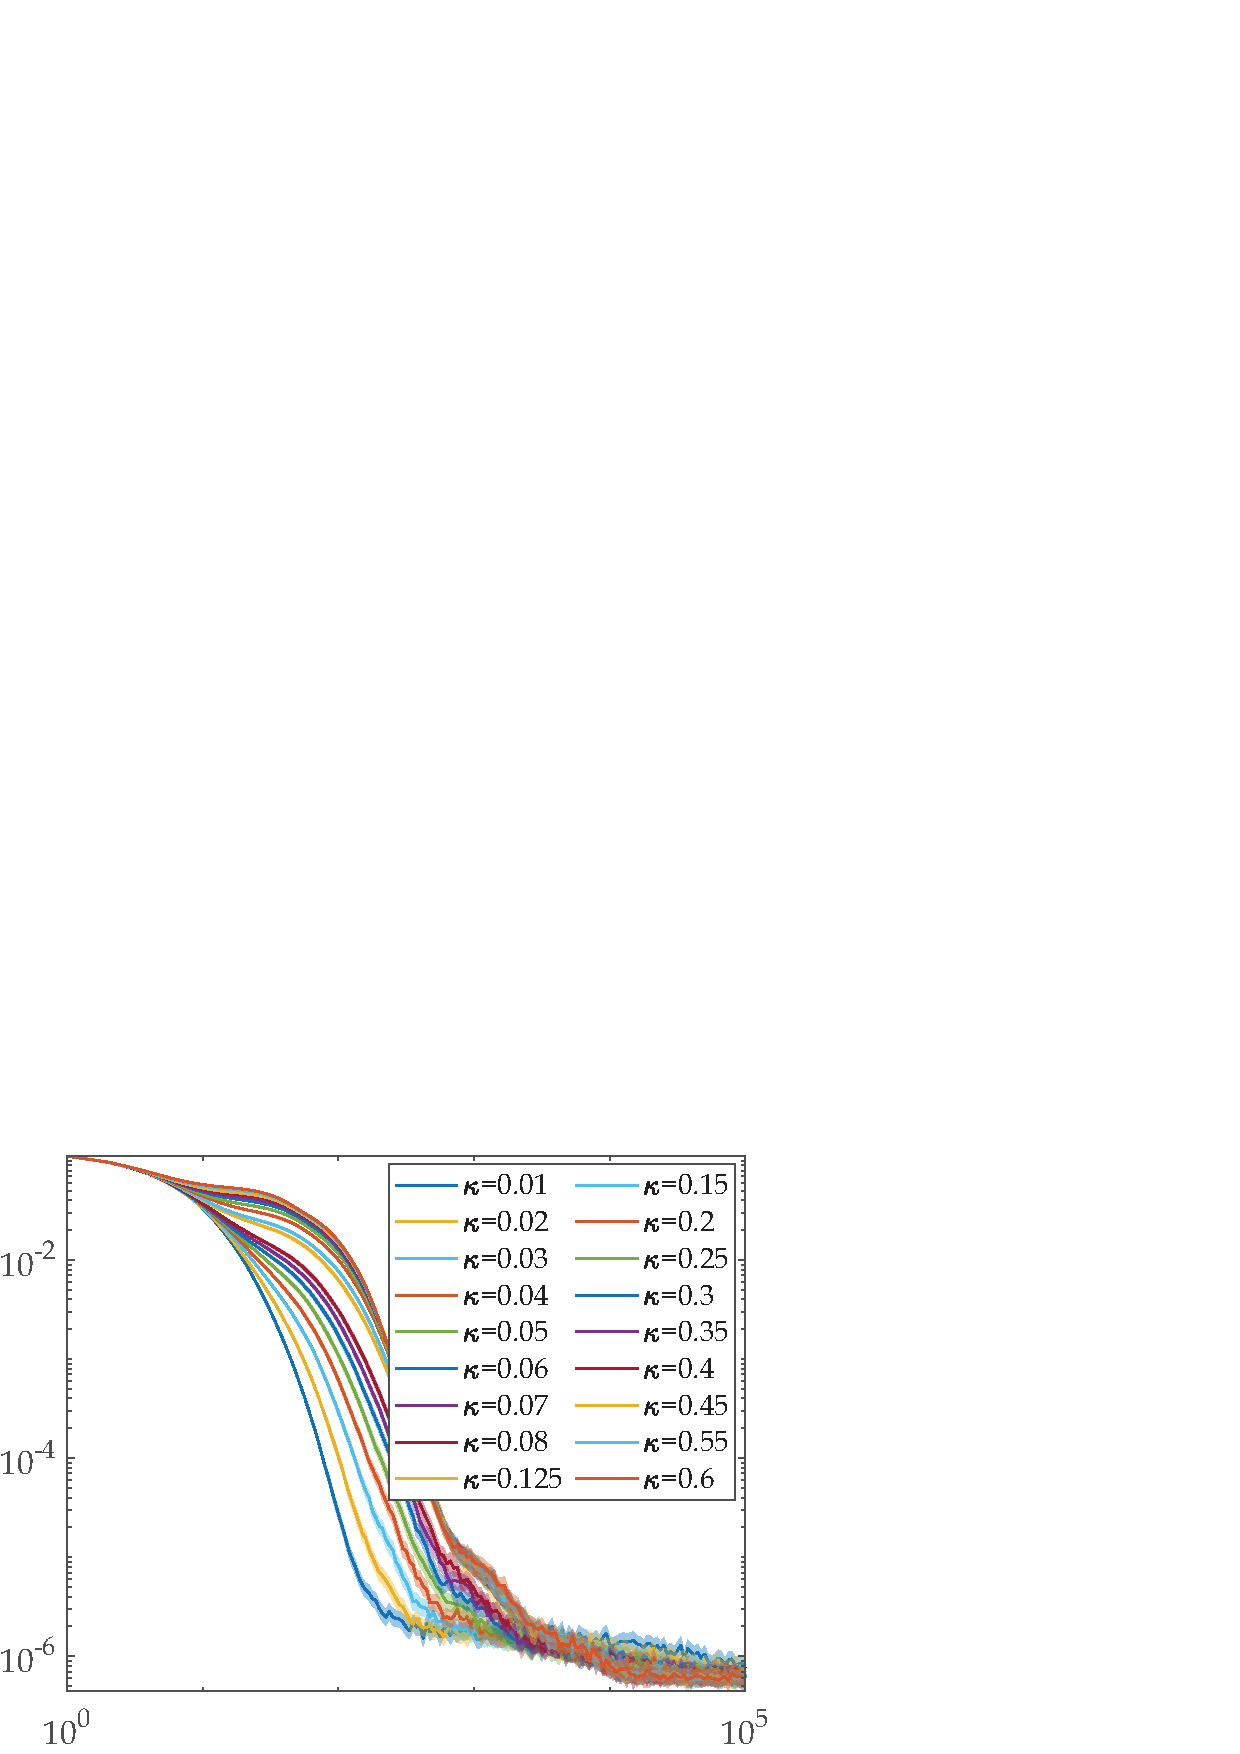
\includegraphics[width=0.6\textwidth]{fig_ringworld_off_1_kappas.pdf}}
\hfill
\subfloat[Sensitivity of $\kappa$ for $\pi_{l}\!=\!0.05$, $b_{l}\!=\!0.15$]{
\captionsetup{justification = centering}
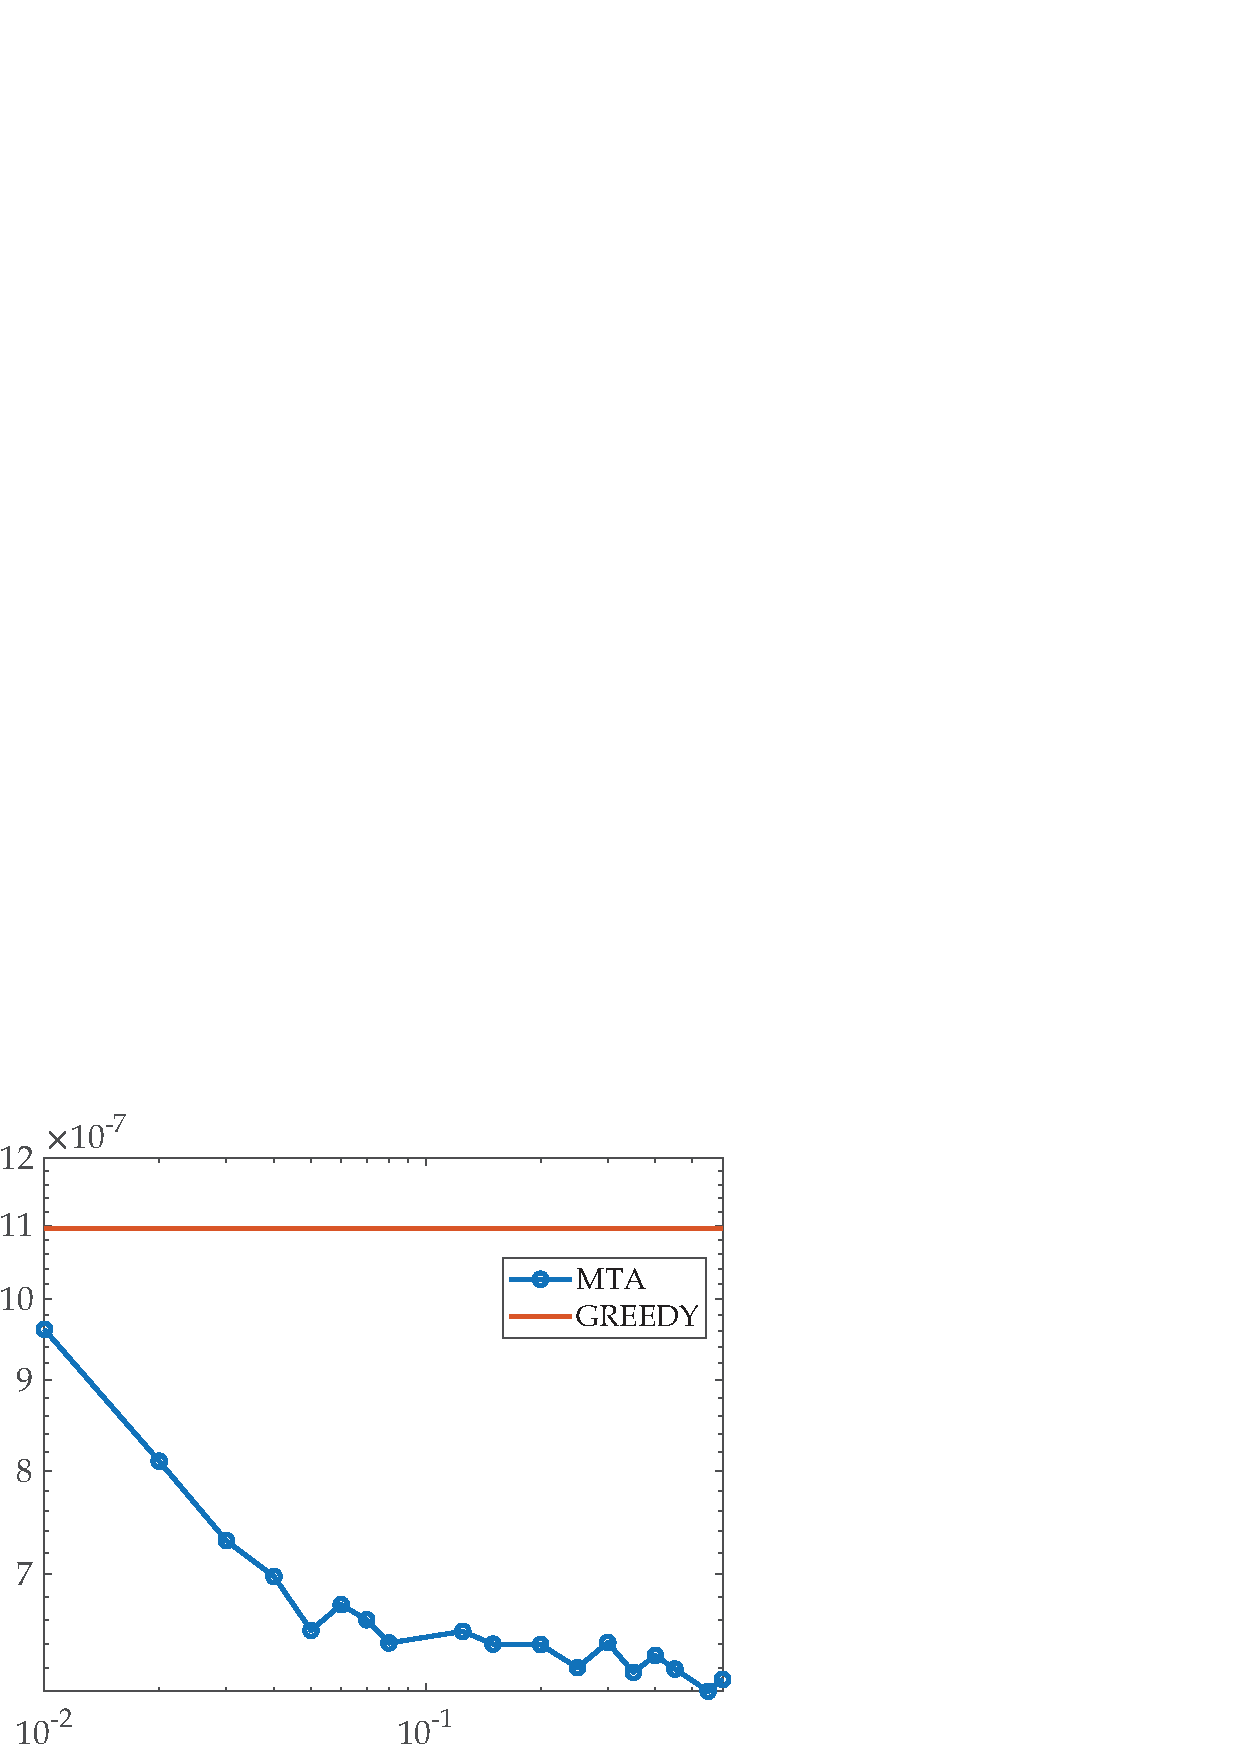
\includegraphics[width=0.6\textwidth]{fig_ringworld_off_1_sensitivity.pdf}}
\end{adjustwidth}
\caption{\small Off-policy error curves of MTA on ringworld with $\alpha = \beta = 0.05$. Each curve or point is averaged from $160$ independent runs.}
\label{fig:ringworld_sensitivity}
\end{figure*}
\par
From the results we can see that MTA is relatively robust in terms of the hyperparameter $\kappa$. When the number of episodes is large, we can safely set $\kappa$ to be a small enough value to achieve good convergence.
\subsection{Frozen Lake: Tests with High Variance}
Ringworlds are low-variance, since the transitions are deterministic and the MDPs are simple. Now we turn to a high-variance environment, the frozenlake, again with binary features. We craft a uniform policy that takes the actions with equal probabilities and a heuristic policy that have $0.3$ probability for going south and east, $0.2$ for going north or west, representing the policy for getting the reward at the southeast corner. We test the on-policy case by setting the behavior and target policies to be the heuristic policy. For off-policy, we use the heuristic as target and the uniform as behavior. The results are presented in Fig. \ref{fig:frozenlake}, alongside with the final errors for different $\kappa$'s.
% \footnote{Walk on the surface of a frozen lake to get our frisbee back. We used Gym FrozenLake-v0. Technically, the environment is not a MDP since it is unsolved also with a trajectory length limit. We get the ground truth by running 30 billion simulations using MC.}
\par
From the results, we observe that greedy and MTA have similar convergence speed but MTA has better accuracy. The sensitivity curves show that in such a high-variance environment, MTA is robust in terms of $\kappa$. Another reason why MTA performs better than greedy on this environment is that the greedy meta-objective of \cite{white2016greedy} is biased towards MC, and thus biased towards environments in which MC performs better, \ie{} the low-variance environments.
\par

\section{Conclusion}
This paper uses the idea of meta-learning to adapt the hyperparameter $\lambda$ during the training of TD($\lambda$) algorithms. Upon existing ideas, we have derived a non-greedy algorithm for \textit{fully} and \textit{truly} optimizing the bias-variance tradeoff of the overall target error, with the help of the $\Lambda$-return variance estimation methods and the true online GTD($\Lambda$) algorithm. The proposed MTA empirically dominates the existing method and the baselines.

% \section*{Acknowledgements}
% We want to express our sincerest gratitute to Sitao Luan, who has been continuously giving us valuable advice. We also want to thank Prof. Doina Precup for her comments and suggestions. Finally, we are grateful for the computational resources on Compute Canada clusters, supported by Mila.

\begin{figure*}
\centering
\begin{adjustwidth}{-1.5in}{-1.5in}
\subfloat[On-policy error with $\kappa = 0.5$]{
\captionsetup{justification = centering}
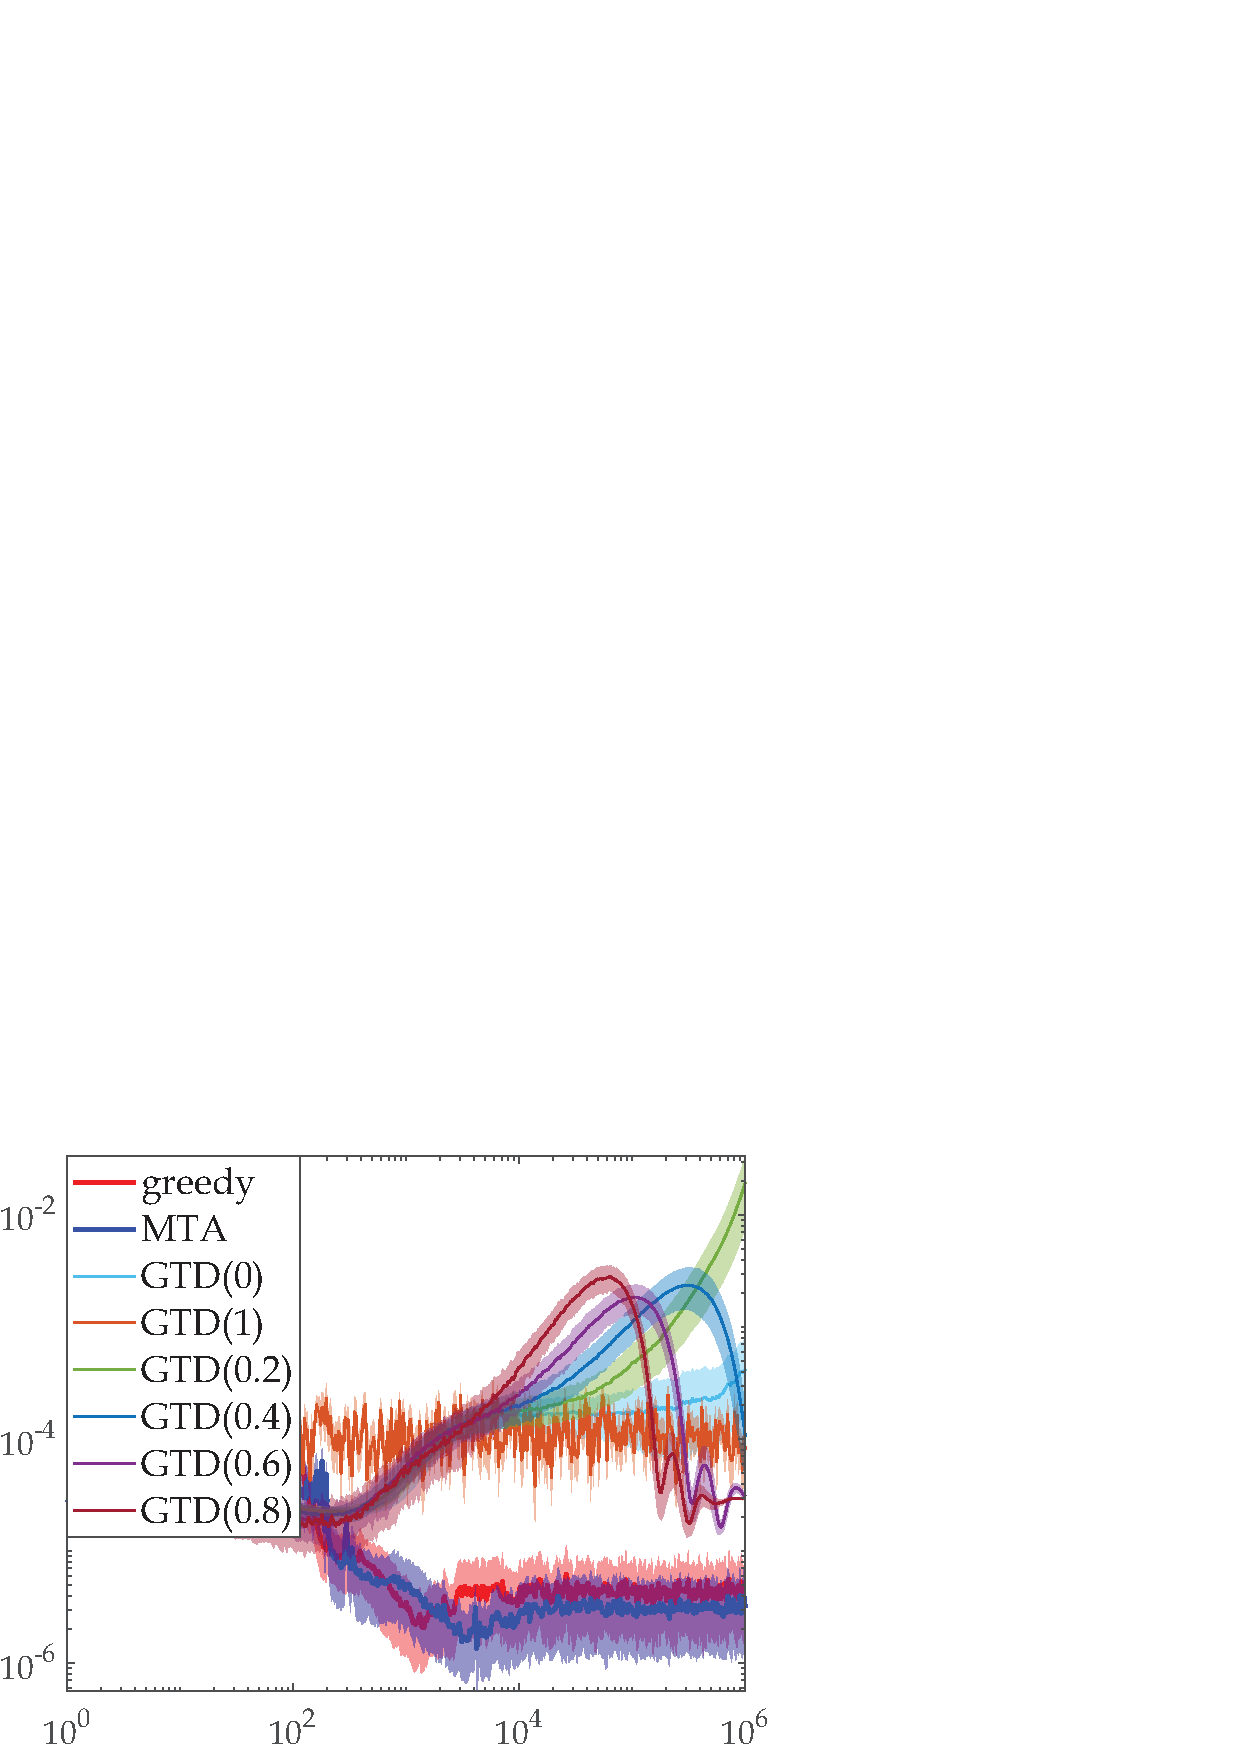
\includegraphics[width=0.37\textwidth]{fig_frozenlake_on_value.pdf}}
\hfill
\subfloat[On-policy sensitivity: x-axis is $\kappa$]{
\captionsetup{justification = centering}
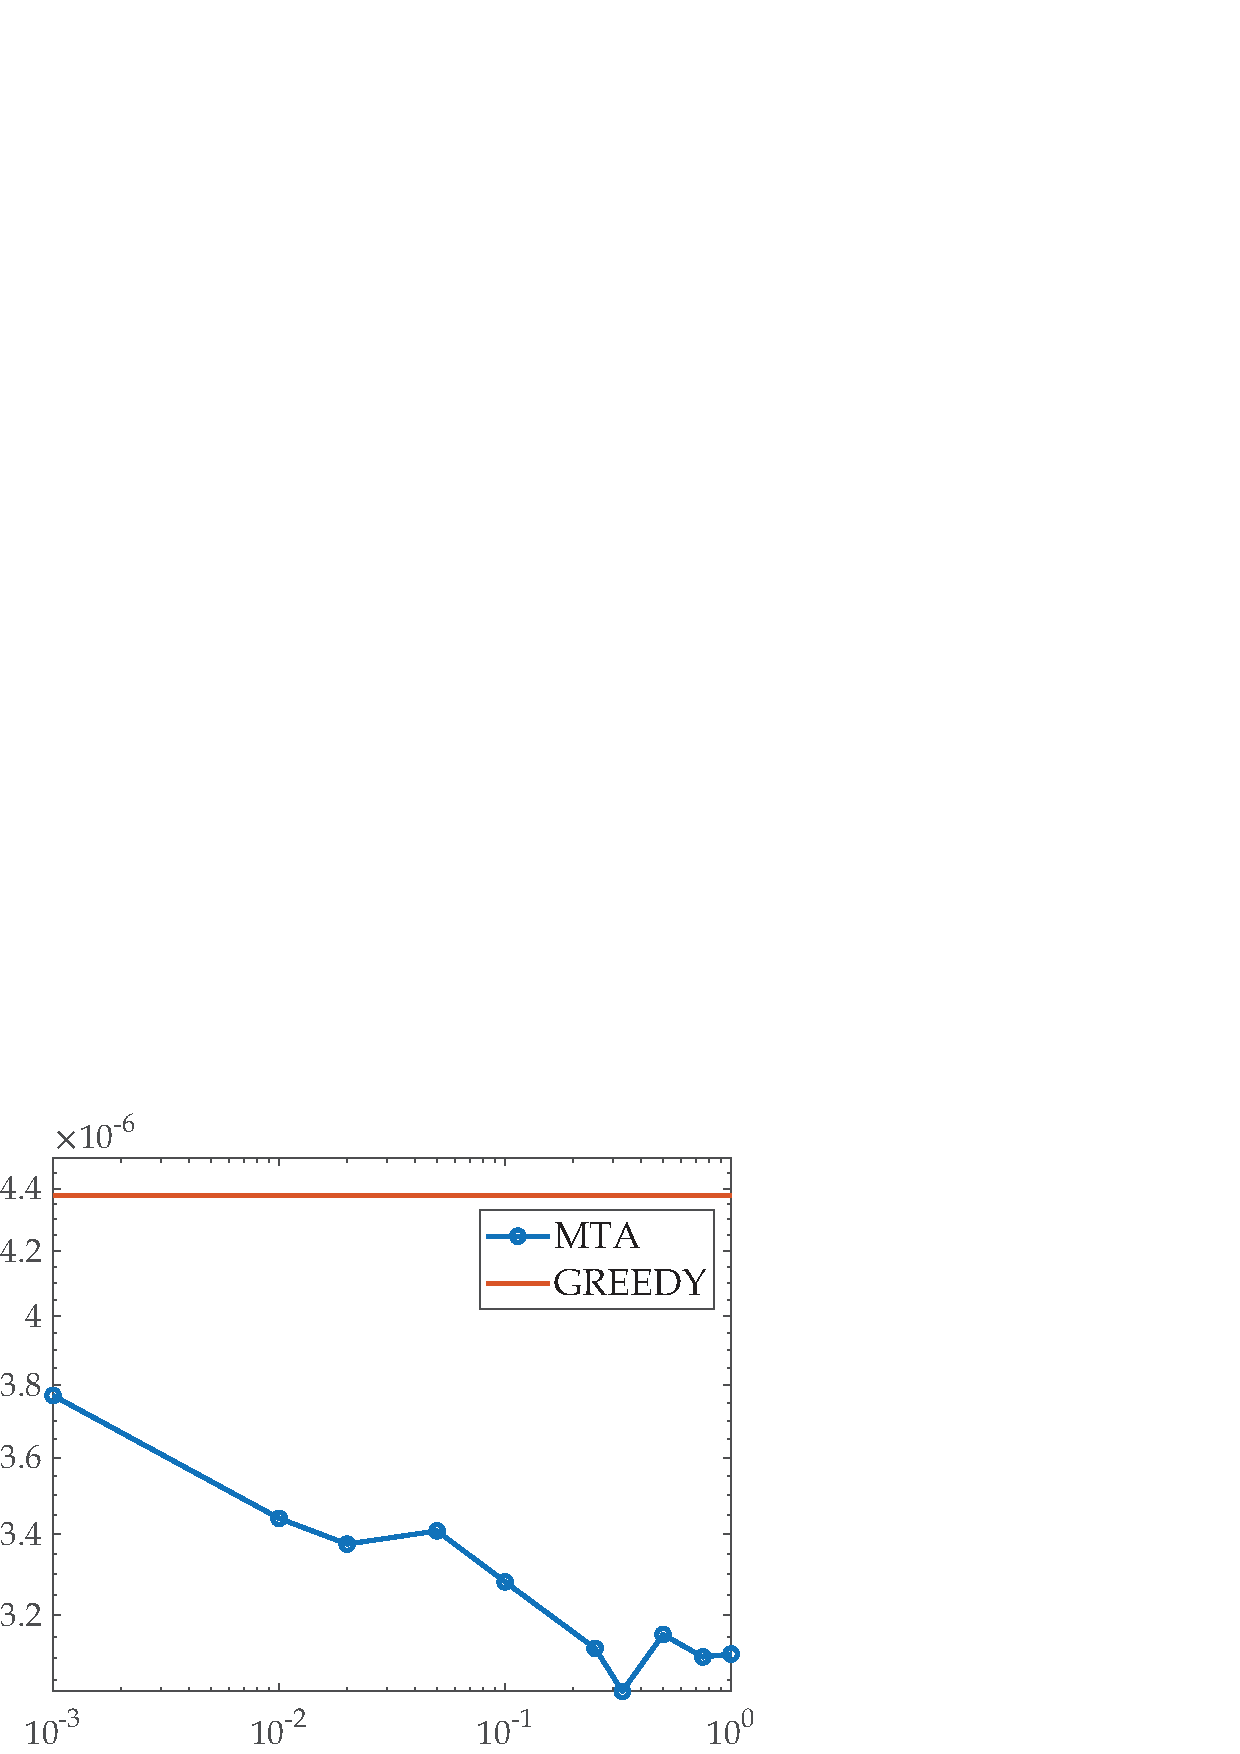
\includegraphics[width=0.37\textwidth]{fig_frozenlake_on_sensitivity.pdf}}
\hfill
\subfloat[Off-policy error with $\kappa = 0.5$]{
\captionsetup{justification = centering}
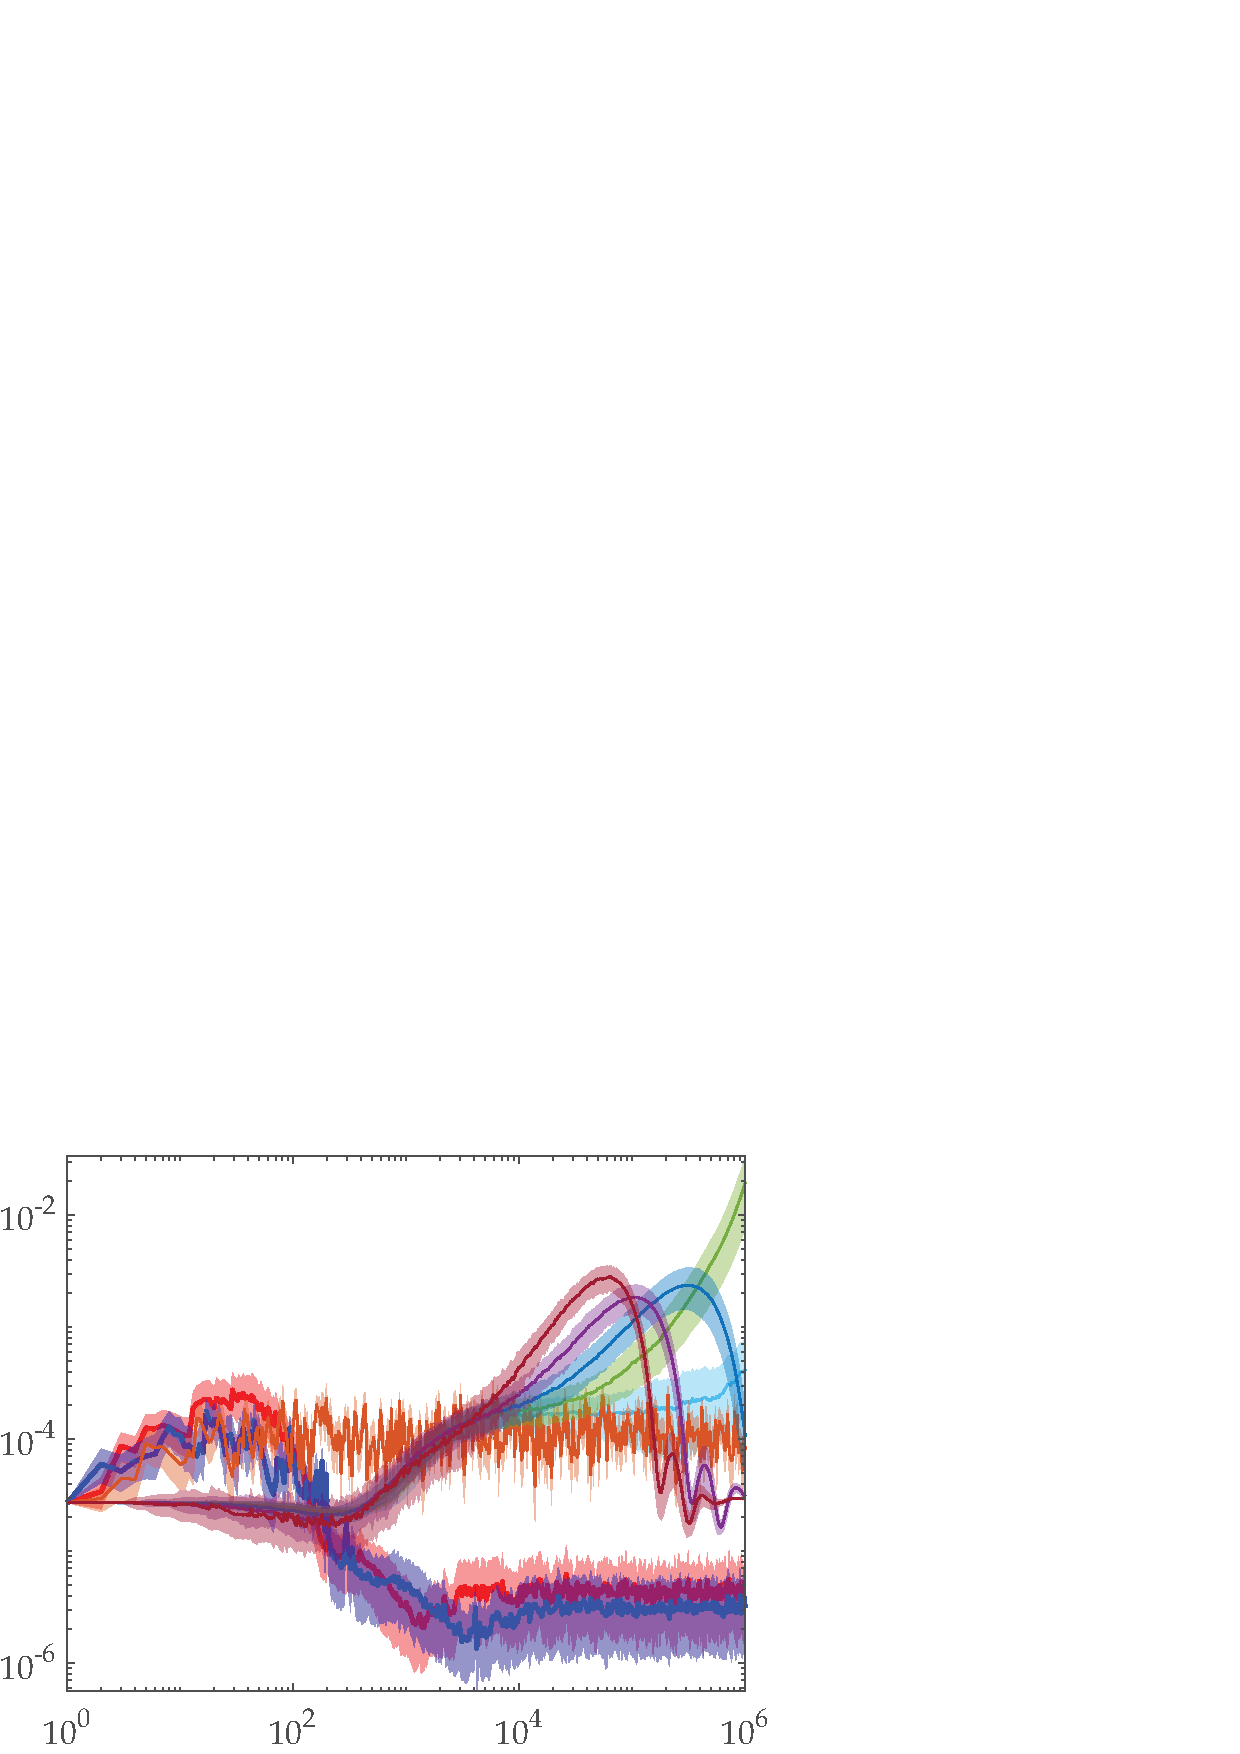
\includegraphics[width=0.37\textwidth]{fig_frozenlake_off_value.pdf}}
\hfill
\subfloat[Off-policy sensitivity]{
\captionsetup{justification = centering}
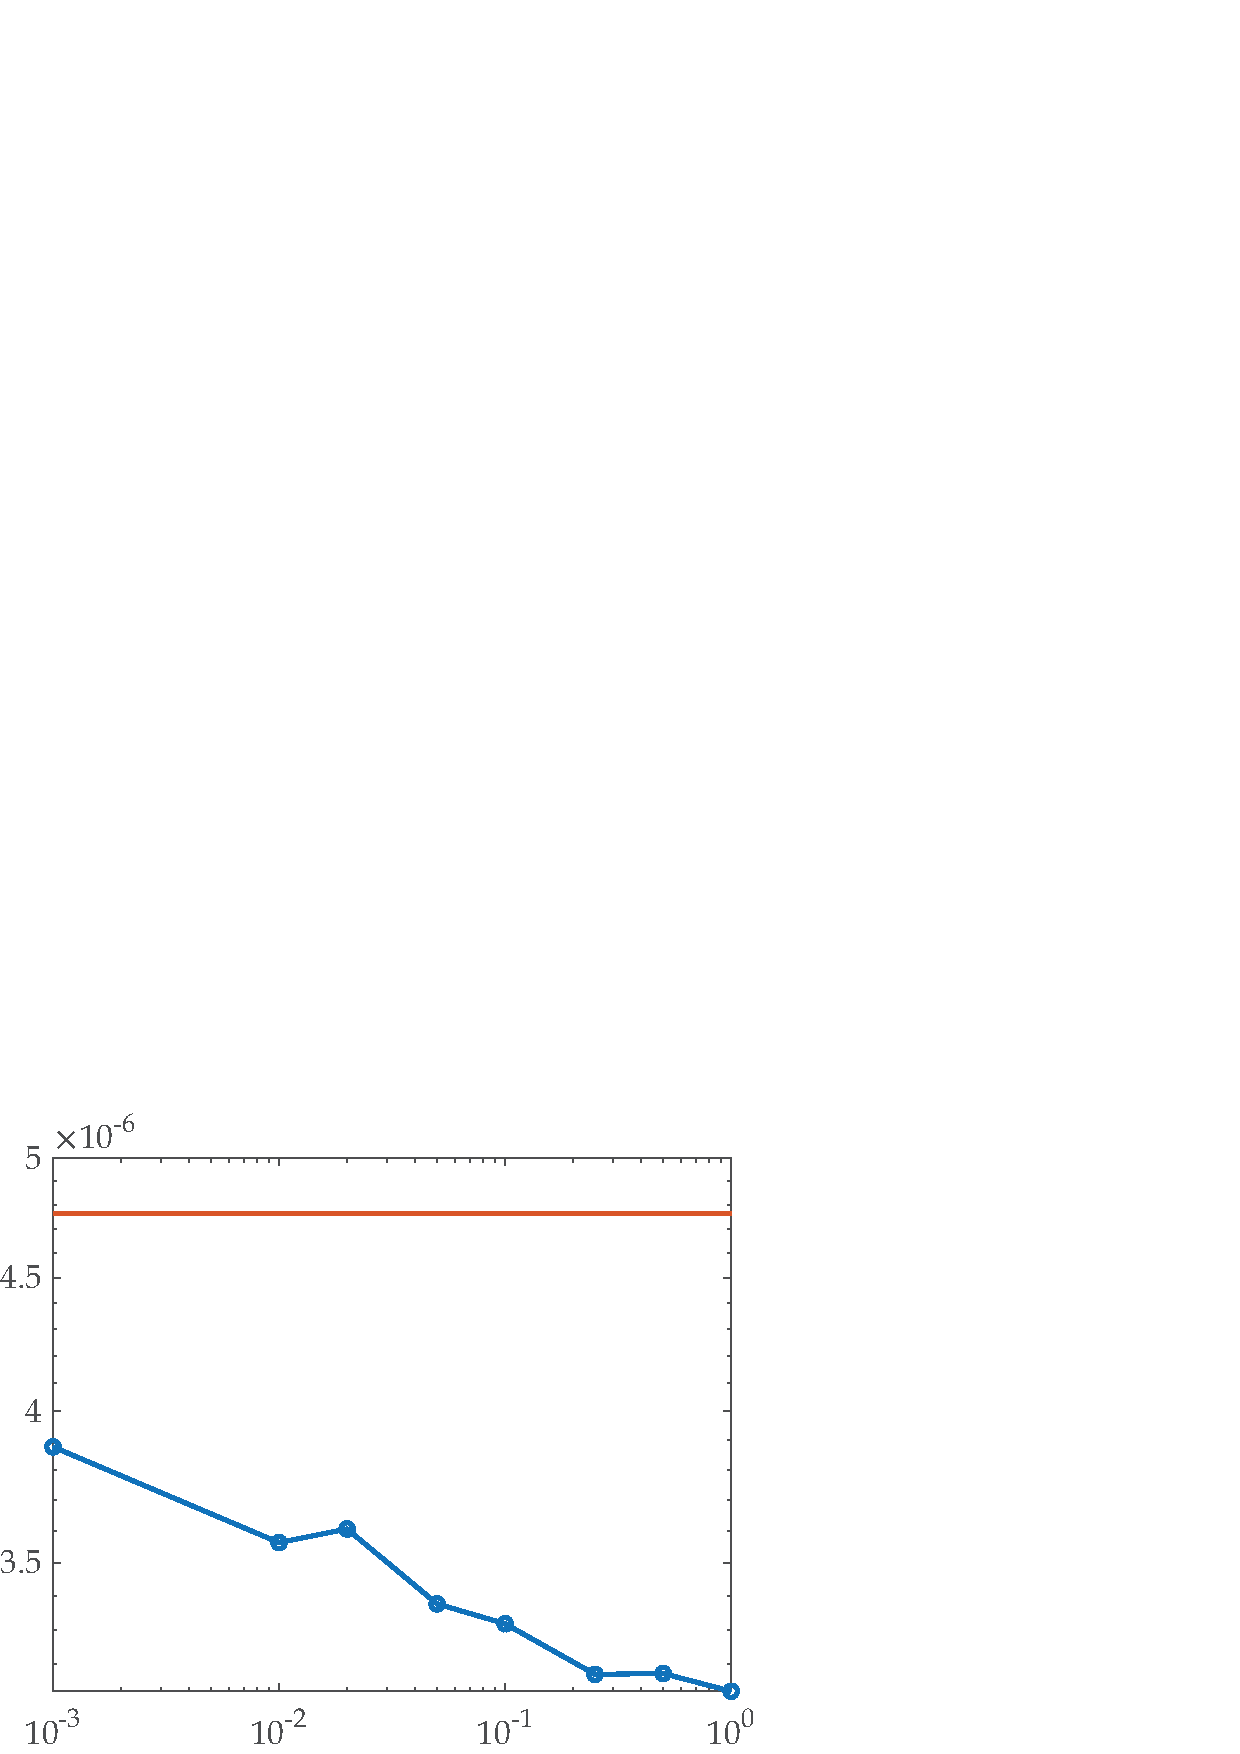
\includegraphics[width=0.37\textwidth]{fig_frozenlake_off_sensitivity.pdf}}
\end{adjustwidth}
\caption{\small Error curves and sensitivity curves on frozenlake with $\alpha = \beta = 0.05$. Results of MTA on the left are with $\kappa = 0.5$. We run $1000000$ episodes for $160$ independent runs. The sensitivity curves on the right show mean final error with different $\kappa$ values.}
\label{fig:frozenlake}
\end{figure*}
\bibliographystyle{IEEEtran}
\bibliography{references}
\newpage

\section*{Appendices}
\subsection{Proof of Proposition \ref{prop:greedy_minimizer}}
\begin{proof}
To minimize the MSE error in terms of $\lambda^{(t+1)}$, we first decompose it:
\begin{proposition}[Minimizer of Greedy Objective]
Given the update target $\hat{G}_t$ of state $s$, the minimizer $\lambda_{(t+1)}^*$ of the mean squared target error of the state
$MSE \equiv \doubleE[{(\hat{G}_t - \doubleE[G_t])}^2]$ is:
\begin{equation}
\lambda_{(t+1)}^* = \frac{{err}^2(\bm{w}^{(t)}, \bm{x}_{t+1})}{Var[G_{t+1}] + {err}^2(\bm{w}^{(t)}, \bm{x}_{t+1})}
\end{equation}
\end{proposition}

\begin{equation}
\begin{aligned}
MSE(\lambda^{(t+1)}) & \equiv \doubleE[{(\hat{G}_t - \doubleE[G_t])}^2]\\
& = \doubleE^2[\hat{G}_t - \doubleE[G_t]] + Var[\hat{G}_t - \doubleE[G_t]] && \text{($Var[Z] = \doubleE[Z^2] + \doubleE^2[Z]$)}\\
& = \doubleE^2[\hat{G}_t - G_t] + Var[\hat{G}_t - \doubleE[G_t]] && \text{(both $\doubleE$ are \wrt{} policy)}\\
& \equiv {Bias}^2(\lambda^{(t+1)}) + {Variance}(\lambda^{(t+1)})
\end{aligned}
\end{equation}

Now we decomposed the objective to the squared bias and the variance. Let us begin by rewriting the bias. Since we have $\bm{x}_t$, $\bm{x}_{t+1}$, $\rho_t$ and $\gamma_{t+1}$,

\begin{equation}
\begin{aligned}
\doubleE[\hat{G}_t] & = \rho_t \doubleE[R_{t+1} + \gamma_{t+1}(1-\lambda^{(t+1)})J(\bm{x}_{t+1}, \bm{w}^{(t)}) + \lambda^{(t+1)} G_{t+1}]\\
& = \rho_t \doubleE[R_{t+1}] + \rho_t \gamma_{t+1} \left((1-\lambda^{(t+1)})J(\bm{x}_{t+1}, \bm{w}^{(t)}) + \lambda^{(t+1)} \doubleE[G_{t+1}]\right)
\end{aligned}
\end{equation}

For convenience, define $err(\bm{w}, \bm{x}_{t+1}) \equiv \doubleE[G_{t+1}] - J(\bm{x}_{t+1}, \bm{w}^{(t)})$ as the difference between the $\lambda = 1$ return and the current approximate value from $\bm{x}_{t+1}$ using weights $\bm{w}^{(t)}$. Using the definition, we can rewrite

\begin{equation}
\begin{aligned}
\doubleE[\hat{G}_t] & = \rho_t \doubleE[R_{t+1}] + \rho_t \gamma_{t+1} \left((1-\lambda^{(t+1)})J(\bm{x}_{t+1}, \bm{w}^{(t)}) + \lambda^{(t+1)} \doubleE[G_{t+1}]\right)\\
& = \doubleE[G_t] - \rho_t \gamma_{t+1} (1-\lambda^{(t+1)})err(\bm{w}^{(t)}, \bm{x}_{t+1})
\end{aligned}
\end{equation}

Thus

\begin{equation}
{Bias}^2(\lambda^{(t+1)}) = \doubleE^2[\hat{G}_t - G_t] = \rho_t^2 \gamma_{t+1}^2 (1 - \lambda^{(t+1)})^2 {err}^2(\bm{w}^{(t)}, \bm{x}_{t+1})
\end{equation}

Assuming the noise in the reward $R_{t+1}$ given $\bm{x}_{t}$ and $\bm{x}_{t+1}$ is independent of other dynamics
\begin{equation}
\begin{aligned}
Variance(\lambda^{(t+1)}) & \equiv Var[\hat{G}_t]\\
& = Var[\rho_t(R_{t+1} + \gamma_{t+1} [(1 - \lambda^{(t+1)})J(\bm{x}_{t+1}, w_v^{(t+1)}) + \lambda^{(t+1)} G_{t+1}])]\\
% & = \rho_t^2 \left(Var[R_{t+1}] + \gamma_{t+1}^2 Var[(1 - \lambda^{(t+1)})J(\bm{x}_{t+1}, w_v^{(t+1)}) + \lambda^{(t+1)} G_{t+1}]\right)\\
& = \rho_t^2Var[R_{t+1}] + \rho_t^2\gamma_{t+1}^2\lambda_{(t+1)}^2 Var[ G_{t+1}]% && \text{$(1 - \lambda^{(t+1)})J(\bm{x}_{t+1}, w_v^{(t+1)})$ has no variance}
\end{aligned}
\end{equation}

Now we can use the derivations to simplify the objective:

\begin{equation}
\begin{aligned}
\lambda_{(t+1)}^* % & = \argmin_{\lambda_{(t+1)} \in [0, 1]}{MSE(\lambda_{(t+1)})}\\
& = \argmin_{\lambda_{(t+1)} \in [0, 1]}{{Bias}^2(\lambda_{(t+1)}) + Variance(\lambda_{(t+1)})}\\
% & = \argmin_{\lambda_{(t+1)} \in [0, 1]}{\rho_t^2 \gamma_{t+1}^2 (1 - \lambda^{(t+1)})^2 {err}^2(\bm{w}^{(t)}, \bm{x}_{t+1}) + \rho_t^2Var[R_{t+1}] + \rho_t^2\gamma_{t+1}^2\lambda_{(t+1)}^2 Var[ G_{t+1}]}\\
& = \argmin_{\lambda_{(t+1)} \in [0, 1]}{(1 - \lambda^{(t+1)})^2 {err}^2(\bm{w}^{(t)}, \bm{x}_{t+1}) + \lambda_{(t+1)}^2 Var[G_{t+1}]} = \frac{{err}^2(\bm{w}^{(t)}, \bm{x}_{t+1})}{Var[G_{t+1}] + {err}^2(\bm{w}^{(t)}, \bm{x}_{t+1})}
\end{aligned}
\end{equation}
\end{proof}


\subsection{Proof of Proposition \ref{prop:objective}}
\begin{proposition}[Gradient of True Objective]
Given the update target $G_t^\Lambda$ of state $s$, the gradient of $MSE \equiv \doubleE[(G_t^\Lambda - \doubleE[G_t])^2]$ is:
\begin{equation}
    \begin{aligned}
    & \nabla_{\lambda^{(t+1)}} \frac{1}{2} MSE(\lambda^{(t+1)}) = \\
    &\gamma_{t+1}^2 \left[\lambda^{(t+1)} \left[ (J(s_{t+1}) - \doubleE[G_{t+1}^\Lambda])^2 + Var[G_{t+1}^\Lambda] \right] + J(s_{t+1})(\doubleE[G_{t+1}^\Lambda] + \doubleE[G_{t+1}]) - J^2(s_{t+1}) - \doubleE[G_{t+1}^\Lambda]\doubleE[G_{t+1}]\right]
    \end{aligned}\nonumber
\end{equation}
And its minimizer is:
\begin{equation}
\begin{aligned}
& \argmin_{\lambda^{(t+1)}}{MSE(\lambda^{(t+1)})} = \frac{J^2(s_{t+1}) + \doubleE[G_{t+1}^\Lambda]\doubleE[G_{t+1}]-J(s_{t+1})(\doubleE[G_{t+1}^\Lambda] + \doubleE[G_{t+1}])}{(J(s_{t+1}) - \doubleE[G_{t+1}^\Lambda])^2 + Var[G_{t+1}^\Lambda]}
\end{aligned}\nonumber
\end{equation}
\end{proposition}

\begin{proof}
\begin{equation}
MSE(\lambda^{(t+1)}) \equiv \doubleE[(G_t^\Lambda - \doubleE[G_t])^2] = \doubleE^2[G_t^\Lambda - G_t] + Var[G_t^\Lambda] \equiv {Bias}^2(\lambda^{(t+1)}) + Variance(\lambda^{(t+1)})
\nonumber
\end{equation}

\begin{equation}
\begin{aligned}
& Variance(\lambda^{(t+1)})\\
& \equiv Var[G_t^\Lambda]\\
& = Var[R_{t+1} + \gamma_{t+1} [(1 - \lambda^{(t+1)})J(s_{t+1}) + \lambda^{(t+1)}G_{t+1}^\Lambda]] && \text{(recursive form)}\\
& = Var[R_{t+1}] + \gamma_{t+1}^2 Var[(1 - \lambda^{(t+1)})J(s_{t+1}) + \lambda^{(t+1)}G_{t+1}^\Lambda]] && \text{($R_{t+1}$ \& $G_{t+1}^\Lambda$ are assumed to be uncorrelated)}\\
& = Var[R_{t+1}] + \gamma_{t+1}^2 \lambda_{(t+1)}^2Var[G_{t+1}^\Lambda] && \text{($(1 - \lambda^{(t+1)})J(s_{t+1})$ not random)}
\end{aligned}
\nonumber
\end{equation}

\begin{equation}
\begin{aligned}
Bias(\lambda^{(t+1)}) & \equiv \doubleE[G_t^\Lambda - G_t]\\
& = \doubleE[R_{t+1} + \gamma_{t+1} [(1 - \lambda^{(t+1)})J(s_{t+1}) + \lambda^{(t+1)}G_{t+1}^\Lambda] - (R_{t+1} + \gamma_{t+1} G_{t+1})] \\
& = \gamma_{t+1} (1 - \lambda^{(t+1)})J(s_{t+1}) + \gamma_{t+1} \lambda^{(t+1)} \doubleE[G_{t+1}^\Lambda] - \gamma_{t+1} \doubleE[G_{t+1}]
\end{aligned}
\nonumber
\end{equation}

\begin{equation}
\begin{aligned}
& \nabla_{\lambda^{(t+1)}} \frac{1}{2} MSE(\lambda^{(t+1)})\\
& \equiv \frac{\bm{\nabla}_{\lambda^{(t+1)}}}{2} \left(\doubleE[(G_t^\Lambda - \doubleE[G_t])^2] \right)\\
& = \frac{\bm{\nabla}_{\lambda^{(t+1)}}}{2} \left(\left(\gamma_{t+1} (1 - \lambda^{(t+1)})J(s_{t+1}) + \gamma_{t+1} \lambda^{(t+1)} \doubleE[G_{t+1}^\Lambda] - \gamma_{t+1} \doubleE[G_{t+1}]\right)^2 + Var[R_{t+1}] + \gamma_{t+1}^2 \lambda_{(t+1)}^2Var[G_{t+1}^\Lambda]\right)\\
& = \gamma_{t+1}^2 \frac{\bm{\nabla}_{\lambda^{(t+1)}}}{2} \left(((1 - \lambda^{(t+1)})J(s_{t+1}) + \lambda^{(t+1)} \doubleE[G_{t+1}^\Lambda] -  \doubleE[G_{t+1}])^2 + \lambda_{(t+1)}^2Var[G_{t+1}^\Lambda]\right)\\
% & = \gamma_{t+1}^2 \frac{\bm{\nabla}_{\lambda^{(t+1)}}}{2} [ \lambda_{(t+1)}^2 \left(
% J^2(s_{t+1}) + \doubleE^2[G_{t+1}^\Lambda] - 2J(s_{t+1})\doubleE[G_{t+1}^\Lambda] + Var[G_{t+1}^\Lambda] \right)\\
% & + \gamma_{t+1}^2  \lambda^{(t+1)} \left(
% -2J^2(s_{t+1}) + 2J(s_{t+1})\doubleE[G_{t+1}^\Lambda] + 2J(s_{t+1})\doubleE[G_{t+1}] - 2\doubleE[G_{t+1}^\Lambda]\doubleE[G_{t+1}]
% \right) ]\\
% & = \lambda^{(t+1)} \left[ J^2(s_{t+1}) + \doubleE^2[G_{t+1}^\Lambda] - 2J(s_{t+1})\doubleE[G_{t+1}^\Lambda] + Var[G_{t+1}^\Lambda] \right] + J(s_{t+1})\doubleE[G_{t+1}^\Lambda] + J(s_{t+1})\doubleE[G_{t+1}]
% -J^2(s_{t+1}) - \doubleE[G_{t+1}^\Lambda]\doubleE[G_{t+1}]\\
& = \gamma_{t+1}^2 \left[\lambda^{(t+1)} \left[ (J(s_{t+1}) - \doubleE[G_{t+1}^\Lambda])^2 + Var[G_{t+1}^\Lambda] \right] + J(s_{t+1})(\doubleE[G_{t+1}^\Lambda] + \doubleE[G_{t+1}]) - J^2(s_{t+1}) - \doubleE[G_{t+1}^\Lambda]\doubleE[G_{t+1}]\right]
\end{aligned}
\nonumber
\end{equation}

The minimizer is achieved by setting the gradient to $0$:
\begin{equation}
\begin{aligned}
& \argmin_{\lambda^{(t+1)}}{MSE(\lambda^{(t+1)})} = \frac{J^2(s_{t+1}) + \doubleE[G_{t+1}^\Lambda]\doubleE[G_{t+1}]-J(s_{t+1})(\doubleE[G_{t+1}^\Lambda] + \doubleE[G_{t+1}])}{(J(s_{t+1}) - \doubleE[G_{t+1}^\Lambda])^2 + Var[G_{t+1}^\Lambda]}
\end{aligned}
\end{equation}
\end{proof}


\subsection{Proof of Theorem \ref{thm:nongreedy}}
\begin{theorem}[Achievement of Optimizing Overall Target Error]
Given an MDP, gradient descent on the true greedy objectives is equivalent to stochastic gradient descent on the overall target MSE for the expected $\Lambda$-return for policy $\pi$, with the assumption that the estimated statistics are accurate. More specifically:
$$\nabla_{\Lambda} \frac{1}{2} MSE(\Lambda) \approx \sum_{s \sim b}{\rho_{acc} \cdot \frac{1}{2} \nabla_{\lambda(s)} MSE(\lambda(s))}$$
where $s$ is the state that the agent is currently experiencing when rolling out behavior policy $b$, $\rho_{acc}$ is the product of all the importance sampling ratios from the beginning of the current episode until meeting state $s$.
\end{theorem}
\begin{proof}
\begin{equation}
\begin{aligned}
\frac{1}{2} MSE(\Lambda) = \sum_{s \in \scriptS}{d_\pi(s) \cdot \frac{1}{2} \doubleE[G^\Lambda(s) - j(s)]^2} \equiv \sum_{s \in \scriptS}{d_\pi(s) \cdot \frac{1}{2} MSE(\lambda(s))}
\end{aligned}\nonumber
\end{equation}

If we take the gradient \wrt{} $\lambda^{(t+1)}$ we can see that:

\begin{equation}
\begin{aligned}
& \nabla_{\Lambda}
\frac{1}{2} MSE(\Lambda)\\
& = \frac{1}{2} \nabla_{\Lambda} \sum_{s \in \scriptS}{d_\pi(s) \cdot MSE(\lambda^{(t+1)})}\\
& =  \frac{1}{2} \nabla_{\Lambda} \sum_{s \in \scriptS}{\sum_{k=0}^{\infty}{\doubleP\{s_0 \to s, k, \pi, s_0 \sim d(s_0) \} MSE(\lambda(s))}}\\
& \text{$\doubleP\{\cdots\}$ is the prob. of $s_0 \to s$ in exactly $k$ steps, $s_0$ is sampled from the starting distribution $d(s_0)$.}\\
& = \frac{1}{2} \nabla_{\Lambda} \sum_{s \in \scriptS}{\sum_{k=0}^{\infty}{\sum_{\tau}{\doubleP\{s_0 \xrightarrow{\tau} s, k, \pi, s_0 \sim d(s_0) \} MSE(\lambda(s))}}}\\
& \text{$\tau$ is a possible trajectory sampled from $s_0$ and transitioning to $s$ with exactly $k$ steps}\\
& = \frac{1}{2} \nabla_{\Lambda} \sum_{s \in \scriptS}{\sum_{k=0}^{\infty}{\sum_{\tau}{p(\tau_0, a_0, \tau_1)\pi(a_0|\tau_0) \cdots p(\tau_{k-1}, a_0, s)\pi(a_{k-1}|\tau_{k-1}) MSE(\lambda(s))}}}\\
& \text{$\tau_i$ is the $i+1$-th state of the trajectory $\tau$ and $p(s, a, s^{'})$ is the probability of $s \xrightarrow{a} s^{'}$ in the MDP}\\
& = \frac{1}{2} \nabla_{\Lambda} \sum_{s \in \scriptS}{\sum_{k=0}^{\infty}{\sum_{\tau}{p(\tau_0, a_0, \tau_1)
\frac{\pi(a_0|\tau_0)}{b(a_0|\tau_0)}
b(a_0|\tau_0)
\cdots p(\tau_{k-1}, a_0, s)
\frac{\pi(a_{k-1}|\tau_{k-1})}{b(a_{k-1}|\tau_{k-1})}
b(a_{k-1}|\tau_{k-1}) MSE(\lambda(s))}}}\\
& \text{inject importance sampling ratios}\\
\end{aligned}\nonumber
\end{equation}
\begin{equation}
\begin{aligned}
& = \frac{1}{2} \nabla_{\Lambda} \sum_{s \in \scriptS}{\sum_{k=0}^{\infty}{\sum_{\tau}{p(\tau_0, a_0, \tau_1) \rho_{0} b(a_0|\tau_0) \cdots p(\tau_{k-1}, a_0, s) \rho_{k-1} b(a_{k-1}|\tau_{k-1}) MSE(\lambda(s))}}}\\
& \text{$\rho_{i} \equiv \frac{\pi(a_i | \tau_i)}{b(a_i | \tau_i)}$ is the importance sampling ratio}\\
& = \frac{1}{2} \nabla_{\Lambda} \sum_{s \in \scriptS}{\sum_{k=0}^{\infty}{\sum_{\tau}{\rho_{0:k-1} \cdot p(\tau_0, a_0, \tau_1)  b(a_0|\tau_0) \cdots p(\tau_{k-1}, a_0, s) b(a_{k-1}|\tau_{k-1}) MSE(\lambda(s))}}}\\
& \text{$\rho_{0:i} \equiv \prod_{j=0}^{i}{\rho_{j}}$ is the importance sampling ratio of the trajectory $\tau$ from $\tau_0$ until $\tau_i$}\\
& = \sum_{s \in \scriptS}{\sum_{k=0}^{\infty}{\sum_{\tau}{\rho_{0:k-1} \cdot p(\tau_0, a_0, \tau_1)  b(a_0|\tau_0) \cdots p(\tau_{k-1}, a_0, s) b(a_{k-1}|\tau_{k-1}) \frac{1}{2} \nabla_{\lambda(s)} MSE(\lambda(s))}}}\\
& \text{the probabilities has nothing to do with $\lambda$, push the gradient inside and $\nabla_{\Lambda}$ becomes $\nabla_{\lambda(s)}$}\\
& \approx \sum_{s \sim b}{\rho_{0:t-1} \cdot \frac{1}{2} \nabla_{\lambda(s)} MSE(\lambda(s))}\\
& \text{the sums are equivalent to summing over the experiencing states driven by $b$}
\end{aligned}\nonumber
\end{equation}
\end{proof}
\subsection{Experiment Details}
\subsubsection{Reproduction of $\lambda$-greedy}
Due to the instability experienced while trying to reproduce the Whites' experiments, we have replaced GTD used in the greedy algorithm with the more stable and robust true online GTD. Also, due to unknown reasons which caused VTD performed extremely unstably, we have replaced the VTD using the direct variance estimation Bellman operator, since they are mathematically equivalent but the latter is more stable and robust empirically. These modifications to the Whites' algorithms are expected only to improve its stability and robustness, without touching the core mechanisms of their algorithm.
\subsubsection{Implementation of MTA}
Due to the instability of the estimates, there could be gradient updates that causes a $\lambda$ value outside the range of $[0, 1]$. In the implementation, whenever we detect such kind of gradient descent step, we simply cancel that operation.

\subsection{Pseudocode of True Online GTD($\Lambda$)}
\begin{algorithm}
\label{alg:true_online_GTD_Lambda}
\caption{True Online GTD($\lambda$) \cite{hasselt2014true}: $\bm{w}^{(t+1)} = togtd(R_{t+1}, \gamma_{t+1},\lambda_{t},\lambda_{t+1},\rho_t)$}
$\delta_t = R_{t+1} + \gamma_{t+1} \bm{x}_{t+1}^T \bm{w}^{(t)} - \bm{x}_{t}^T \bm{w}^{(t)}$;\\
$\bm{z}_t = \rho_t \left[\gamma_t \lambda^{(t)} \bm{z}_{t-1} + \alpha_t (1 - \rho_t \gamma_t \lambda^{(t)} \bm{z}_{t-1}^T\bm{x}_{t}) \bm{x}_{t} \right]$;\\
$\bm{z}_t^\nabla = \rho_t \left[ \gamma_t \lambda^{(t)} \bm{z}_{t-1}^\nabla + \bm{x}_{t} \right]$;\\
$\bm{z}_t^{\bm{h}} = \rho_{t-1} \gamma_t \lambda^{(t)} \bm{z}_{t-1}^{\bm{h}} + \beta_t (1 - \rho_{t-1} \gamma_t \lambda^{(t)} \bm{x}_{t}^T \bm{z}_{t-1}^{\bm{h}})\bm{x}_{t}^T$;\\
$\bm{w}^{(t+1)} = \bm{w}^{(t)} + \delta_t \bm{z}_t + (\bm{w}^{(t)} - \bm{w}^{(t-1)})^T \bm{x}_t(\bm{z}_t - \alpha_t \rho_t \bm{x}_t) - \alpha_t \gamma_{t+1}(1-\lambda^{(t+1)})\bm{h}_t^T \bm{z}_t^\nabla \bm{x}_{t+1}$;\\
$\bm{h}_{t+1} = \bm{h}_{t} + \rho_t \delta_t \bm{z}_t^{\bm{h}} - \beta_t \bm{x}_t^T\bm{h}_{t}\bm{x}_t$;\\
\end{algorithm}
\subsection{On-policy Test Results on Ringworld}
\begin{figure*}
\centering
\begin{adjustwidth}{-1.2in}{-1.2in}
\subfloat[$\pi_{l}\!=b_{l}\!=\!0.05$]{
\captionsetup{justification = centering}
\includegraphics[width=0.45\textwidth]{fig_ringworld_on_1_value.pdf}}
\hfill
\subfloat[$\pi_{l}\!=b_{l}\!=\!0.25$]{
\captionsetup{justification = centering}
\includegraphics[width=0.45\textwidth]{fig_ringworld_on_2_value.pdf}}
\hfill
\subfloat[$\pi_{l}\!=b_{l}\!=\!0.4$]{
\captionsetup{justification = centering}
\includegraphics[width=0.45\textwidth]{fig_ringworld_on_3_value.pdf}}
\end{adjustwidth}
\caption{\small On-policy tests on $\gamma = 0.95$ ringworlds.}
\label{fig:ringworld_on}
\end{figure*}

\subsection{$\lambda$ Curves for Tests}
MTA compared to the greedy algorithm: sometimes $\lambda$ converges to zero quickly; Sometimes it bounces and stay relatively high and sometimes it chatters. We think this is a good sign since we are optimizing $\Lambda$ slowly and one $\lambda$ changes along with the changes of the others.
\begin{figure*}
\centering
\begin{adjustwidth}{-1.2in}{-1.2in}
\subfloat[$\pi_{l}\!=\!0.05$, $b_{l}\!=\!0.15$]{
\captionsetup{justification = centering}
\includegraphics[width=0.45\textwidth]{fig_ringworld_off_1_lambda.pdf}}
\hfill
\subfloat[$\pi_{l}\!=\!0.25$, $b_{l}\!=\!0.33$]{
\captionsetup{justification = centering}
\includegraphics[width=0.45\textwidth]{fig_ringworld_off_2_lambda.pdf}}
\hfill
\subfloat[$\pi_{l}\!=\!0.4$, $b_{l}\!=\!0.5$]{
\captionsetup{justification = centering}
\includegraphics[width=0.45\textwidth]{fig_ringworld_off_3_lambda.pdf}}

\subfloat[$\pi_{l}\!=b_{l}\!=\!0.05$]{
\captionsetup{justification = centering}
\includegraphics[width=0.45\textwidth]{fig_ringworld_on_1_lambda.pdf}}
\hfill
\subfloat[$\pi_{l}\!=b_{l}\!=\!0.25$]{
\captionsetup{justification = centering}
\includegraphics[width=0.45\textwidth]{fig_ringworld_on_2_lambda.pdf}}
\hfill
\subfloat[$\pi_{l}\!=b_{l}\!=\!0.4$]{
\captionsetup{justification = centering}
\includegraphics[width=0.45\textwidth]{fig_ringworld_on_3_lambda.pdf}}
\end{adjustwidth}
\caption{\small $\lambda(s_0)$ on $\gamma = 0.95$ ringworlds.}
\label{fig:ringworld_lambda}
\end{figure*}
% http://web.mit.edu/jnt/www/Papers/J063-97-bvr-td.pdf
\end{document}